\documentclass[twoside]{book}

% Packages required by doxygen
\usepackage{calc}
\usepackage{doxygen}
\usepackage{graphicx}
\usepackage[utf8]{inputenc}
\usepackage{makeidx}
\usepackage{multicol}
\usepackage{multirow}
\usepackage{textcomp}
\usepackage[table]{xcolor}

% Font selection
\usepackage[T1]{fontenc}
\usepackage{mathptmx}
\usepackage[scaled=.90]{helvet}
\usepackage{courier}
\usepackage{amssymb}
\usepackage{sectsty}
\renewcommand{\familydefault}{\sfdefault}
\allsectionsfont{%
  \fontseries{bc}\selectfont%
  \color{darkgray}%
}
\renewcommand{\DoxyLabelFont}{%
  \fontseries{bc}\selectfont%
  \color{darkgray}%
}

% Page & text layout
\usepackage{geometry}
\geometry{%
  a4paper,%
  top=2.5cm,%
  bottom=2.5cm,%
  left=2.5cm,%
  right=2.5cm%
}
\tolerance=750
\hfuzz=15pt
\hbadness=750
\setlength{\emergencystretch}{15pt}
\setlength{\parindent}{0cm}
\setlength{\parskip}{0.2cm}
\makeatletter
\renewcommand{\paragraph}{%
  \@startsection{paragraph}{4}{0ex}{-1.0ex}{1.0ex}{%
    \normalfont\normalsize\bfseries\SS@parafont%
  }%
}
\renewcommand{\subparagraph}{%
  \@startsection{subparagraph}{5}{0ex}{-1.0ex}{1.0ex}{%
    \normalfont\normalsize\bfseries\SS@subparafont%
  }%
}
\makeatother

% Headers & footers
\usepackage{fancyhdr}
\pagestyle{fancyplain}
\fancyhead[LE]{\fancyplain{}{\bfseries\thepage}}
\fancyhead[CE]{\fancyplain{}{}}
\fancyhead[RE]{\fancyplain{}{\bfseries\leftmark}}
\fancyhead[LO]{\fancyplain{}{\bfseries\rightmark}}
\fancyhead[CO]{\fancyplain{}{}}
\fancyhead[RO]{\fancyplain{}{\bfseries\thepage}}
\fancyfoot[LE]{\fancyplain{}{}}
\fancyfoot[CE]{\fancyplain{}{}}
\fancyfoot[RE]{\fancyplain{}{\bfseries\scriptsize Generated on Sat Jan 31 2015 04\-:48\-:56 for Bixel by Doxygen }}
\fancyfoot[LO]{\fancyplain{}{\bfseries\scriptsize Generated on Sat Jan 31 2015 04\-:48\-:56 for Bixel by Doxygen }}
\fancyfoot[CO]{\fancyplain{}{}}
\fancyfoot[RO]{\fancyplain{}{}}
\renewcommand{\footrulewidth}{0.4pt}
\renewcommand{\chaptermark}[1]{%
  \markboth{#1}{}%
}
\renewcommand{\sectionmark}[1]{%
  \markright{\thesection\ #1}%
}

% Indices & bibliography
\usepackage{natbib}
\usepackage[titles]{tocloft}
\setcounter{tocdepth}{3}
\setcounter{secnumdepth}{5}
\makeindex

% Hyperlinks (required, but should be loaded last)
\usepackage{ifpdf}
\ifpdf
  \usepackage[pdftex,pagebackref=true]{hyperref}
\else
  \usepackage[ps2pdf,pagebackref=true]{hyperref}
\fi
\hypersetup{%
  colorlinks=true,%
  linkcolor=blue,%
  citecolor=blue,%
  unicode%
}

% Custom commands
\newcommand{\clearemptydoublepage}{%
  \newpage{\pagestyle{empty}\cleardoublepage}%
}


%===== C O N T E N T S =====

\begin{document}

% Titlepage & ToC
\hypersetup{pageanchor=false}
\pagenumbering{roman}
\begin{titlepage}
\vspace*{7cm}
\begin{center}%
{\Large Bixel }\\
\vspace*{1cm}
{\large Generated by Doxygen 1.8.6}\\
\vspace*{0.5cm}
{\small Sat Jan 31 2015 04:48:56}\\
\end{center}
\end{titlepage}
\clearemptydoublepage
\tableofcontents
\clearemptydoublepage
\pagenumbering{arabic}
\hypersetup{pageanchor=true}

%--- Begin generated contents ---
\chapter{Todo List}
\label{todo}
\hypertarget{todo}{}

\begin{DoxyRefList}
\item[\label{todo__todo000003}%
\hypertarget{todo__todo000003}{}%
Member \hyperlink{classBixelGrid_a3980df6f8699db73452b0893190877ce}{Bixel\-Grid\-:\-:decrease\-Dimension} ()]Get rid of this. See the todos in \#increase\-Dimension.  
\item[\label{todo__todo000001}%
\hypertarget{todo__todo000001}{}%
Member \hyperlink{classBixelGrid_aac761dbec07e93c105dd7332e982698c}{Bixel\-Grid\-:\-:dimension} ()]Get rid of this. See \#increase\-Dimension todos.  
\item[\label{todo__todo000005}%
\hypertarget{todo__todo000005}{}%
Member \hyperlink{classBixelGrid_a2f45709d9159599eb3af5ceed54fc550}{Bixel\-Grid\-:\-:Draw\-Tool} ]Move H\-A\-N\-D and Z\-O\-O\-M to an enum in \hyperlink{classCanvasWidget}{Canvas\-Widget}. 

Implement E\-Y\-E\-D\-R\-O\-P 

Add a Paint\-Bucket tool. 

Add a Magic wand tool. 

Flesh out tools enum documentation  
\item[\label{todo__todo000002}%
\hypertarget{todo__todo000002}{}%
Member \hyperlink{classBixelGrid_a589e8542077e6afea967a85e8d040298}{Bixel\-Grid\-:\-:increase\-Dimension} ()]The way I have been dealing with \#dimension is ridiculous. Get rid of m\-\_\-dimension altogether and use only \#grid\-Width and \#grid\-Height. Create an increase\-Width() and an increase\-Height() as well as a decrease\-Width/\-Height.  
\item[\label{todo__todo000006}%
\hypertarget{todo__todo000006}{}%
Member \hyperlink{classBixelGrid_a2f45709d9159599eb3af5ceed54fc550aa9b97045f133062453e585409323d940}{Bixel\-Grid\-:\-:P\-A\-I\-N\-T\-B\-U\-C\-K\-E\-T} ]implement this  
\item[\label{todo__todo000004}%
\hypertarget{todo__todo000004}{}%
Member \hyperlink{classBixelGrid_a5ddc685a7df1db41dd1716e03342d619}{Bixel\-Grid\-:\-:paint\-G\-L} ()]Give Bixel drawing work to Open\-G\-L. Use one Mesh instead of many calls to G\-L\-\_\-\-D\-R\-A\-W\-\_\-\-A\-R\-R\-A\-Y\-S  
\item[\label{todo__todo000007}%
\hypertarget{todo__todo000007}{}%
Class \hyperlink{classBixelWindow}{Bixel\-Window} ]Figure out how to keep focus on gl\-Widget. Maybe make al gl\-Widget keyboard actions Q\-Actions in the menu? 
\end{DoxyRefList}
\chapter{Current tasks}
\label{task}
\hypertarget{task}{}

\begin{DoxyRefList}
\item[\label{task__task000001}%
\hypertarget{task__task000001}{}%
Class \hyperlink{classGLWidget}{G\-L\-Widget} ]Adding a m\-\_\-marked\-Bixels vector that will contain every Bixel that has been changed since the last call to \#paint\-G\-L.
\begin{DoxyItemize}
\item Create the member variable $\ast$$\ast$$\ast$
\item Create a mark\-Bixel(int i, int j) method
\item Go through every mutator of \#color\-Matrix and add a call to mark\-Bixel(int i, int j)
\item Update paint\-G\-L to draw only the bixels that have been marked. 
\end{DoxyItemize}
\end{DoxyRefList}
\chapter{Todo high priority list}
\label{todo1}
\hypertarget{todo1}{}

\begin{DoxyRefList}
\item[\label{todo1__todo1000001}%
\hypertarget{todo1__todo1000001}{}%
Class \hyperlink{classGLWidget}{G\-L\-Widget} ]Make sure delicate members like m\-\_\-color\-Matrix and m\-\_\-selected\-Bixels are only accessed through accessor and mutator methods. 
\end{DoxyRefList}
\chapter{Hierarchical Index}
\section{Class Hierarchy}
This inheritance list is sorted roughly, but not completely, alphabetically\-:\begin{DoxyCompactList}
\item \contentsline{section}{Bixel\-Grid\-:\-:History\-State}{\pageref{structBixelGrid_1_1HistoryState}}{}
\item Q\-G\-L\-Widget\begin{DoxyCompactList}
\item \contentsline{section}{Bixel\-Grid}{\pageref{classBixelGrid}}{}
\end{DoxyCompactList}
\item Q\-Main\-Window\begin{DoxyCompactList}
\item \contentsline{section}{Bixel\-Window}{\pageref{classBixelWindow}}{}
\end{DoxyCompactList}
\item Q\-Tool\-Button\begin{DoxyCompactList}
\item \contentsline{section}{Swatch}{\pageref{classSwatch}}{}
\end{DoxyCompactList}
\item Q\-Widget\begin{DoxyCompactList}
\item \contentsline{section}{Canvas\-Widget}{\pageref{classCanvasWidget}}{}
\end{DoxyCompactList}
\item \contentsline{section}{vec2}{\pageref{classvec2}}{}
\end{DoxyCompactList}

\chapter{Class Index}
\section{Class List}
Here are the classes, structs, unions and interfaces with brief descriptions\-:\begin{DoxyCompactList}
\item\contentsline{section}{\hyperlink{classBixelWindow}{Bixel\-Window} }{\pageref{classBixelWindow}}{}
\item\contentsline{section}{\hyperlink{classCanvasWidget}{Canvas\-Widget} }{\pageref{classCanvasWidget}}{}
\item\contentsline{section}{\hyperlink{classGLWidget}{G\-L\-Widget} \\*A Widget for rendering and drawing Bixels }{\pageref{classGLWidget}}{}
\item\contentsline{section}{\hyperlink{structGLWidget_1_1HistoryState}{G\-L\-Widget\-::\-History\-State} \\*This struct stores the current state of a \hyperlink{classGLWidget}{G\-L\-Widget} }{\pageref{structGLWidget_1_1HistoryState}}{}
\item\contentsline{section}{\hyperlink{classSwatch}{Swatch} }{\pageref{classSwatch}}{}
\item\contentsline{section}{\hyperlink{classvec2}{vec2} }{\pageref{classvec2}}{}
\end{DoxyCompactList}

\chapter{Class Documentation}
\hypertarget{classBixelWindow}{\section{Bixel\-Window Class Reference}
\label{classBixelWindow}\index{Bixel\-Window@{Bixel\-Window}}
}


{\ttfamily \#include $<$bixelwindow.\-hpp$>$}



Inheritance diagram for Bixel\-Window\-:\nopagebreak
\begin{figure}[H]
\begin{center}
\leavevmode
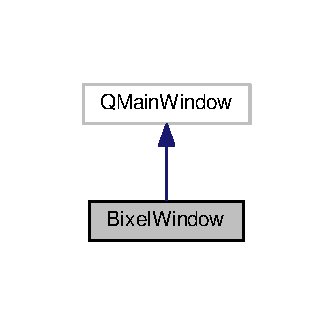
\includegraphics[width=160pt]{classBixelWindow__inherit__graph}
\end{center}
\end{figure}


Collaboration diagram for Bixel\-Window\-:\nopagebreak
\begin{figure}[H]
\begin{center}
\leavevmode
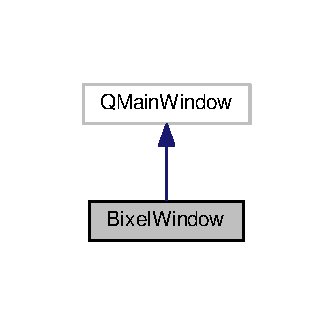
\includegraphics[width=160pt]{classBixelWindow__coll__graph}
\end{center}
\end{figure}
\subsection*{Public Slots}
\begin{DoxyCompactItemize}
\item 
\hypertarget{classBixelWindow_a4cb74f4db84d75a09598acba37f97268}{void {\bfseries open\-\_\-slot} (std\-::string file\-Name)}\label{classBixelWindow_a4cb74f4db84d75a09598acba37f97268}

\end{DoxyCompactItemize}
\subsection*{Signals}
\begin{DoxyCompactItemize}
\item 
\hypertarget{classBixelWindow_a0ca7305900c3368348c36dbd73a51af9}{void {\bfseries new\-\_\-file\-\_\-signal} ()}\label{classBixelWindow_a0ca7305900c3368348c36dbd73a51af9}

\item 
\hypertarget{classBixelWindow_ac3542a30d554c494749f81c4928e4691}{void {\bfseries save\-\_\-signal} ()}\label{classBixelWindow_ac3542a30d554c494749f81c4928e4691}

\item 
\hypertarget{classBixelWindow_a184916c5970b4189571c61a40bcddb81}{void {\bfseries save\-\_\-as\-\_\-signal} (const std\-::string \&file\-Name)}\label{classBixelWindow_a184916c5970b4189571c61a40bcddb81}

\item 
\hypertarget{classBixelWindow_a1f5cdec267152e7c84fa3430c4cea442}{void {\bfseries open\-\_\-signal} (const std\-::string \&file\-Name)}\label{classBixelWindow_a1f5cdec267152e7c84fa3430c4cea442}

\item 
\hypertarget{classBixelWindow_a64703a78a6b4e436248dbed135fe5420}{void {\bfseries export\-\_\-image\-\_\-signal} (const std\-::string \&file\-Name)}\label{classBixelWindow_a64703a78a6b4e436248dbed135fe5420}

\item 
\hypertarget{classBixelWindow_af52996e623d4b53b5dc905c931960dc1}{void {\bfseries preferences\-\_\-signal} ()}\label{classBixelWindow_af52996e623d4b53b5dc905c931960dc1}

\item 
\hypertarget{classBixelWindow_a94c52d6d03787661d8cb142657cfebbd}{void {\bfseries undo\-\_\-signal} ()}\label{classBixelWindow_a94c52d6d03787661d8cb142657cfebbd}

\item 
\hypertarget{classBixelWindow_aaec5ff0c79673adf41f9d11acf8d696d}{void {\bfseries redo\-\_\-signal} ()}\label{classBixelWindow_aaec5ff0c79673adf41f9d11acf8d696d}

\item 
\hypertarget{classBixelWindow_a752d221cb9e200ee23a3ad0cf20fd8b8}{void {\bfseries copy\-\_\-signal} ()}\label{classBixelWindow_a752d221cb9e200ee23a3ad0cf20fd8b8}

\item 
\hypertarget{classBixelWindow_a1fe8ae25f04273997c5b23bbb161af4e}{void {\bfseries cut\-\_\-signal} ()}\label{classBixelWindow_a1fe8ae25f04273997c5b23bbb161af4e}

\item 
\hypertarget{classBixelWindow_a587d0745d036eabace33de931104d4c7}{void {\bfseries paste\-\_\-signal} ()}\label{classBixelWindow_a587d0745d036eabace33de931104d4c7}

\item 
\hypertarget{classBixelWindow_a42b6e8b3cc3f837a6233c616ea26a9c4}{void {\bfseries select\-\_\-all\-\_\-signal} ()}\label{classBixelWindow_a42b6e8b3cc3f837a6233c616ea26a9c4}

\item 
\hypertarget{classBixelWindow_a5e64c14663eadc91c7c6015d4981fb70}{void {\bfseries deselect\-\_\-all\-\_\-signal} ()}\label{classBixelWindow_a5e64c14663eadc91c7c6015d4981fb70}

\item 
\hypertarget{classBixelWindow_a119d72d0e838a8d3689a3adecd4525e4}{void {\bfseries reset\-\_\-view\-\_\-signal} ()}\label{classBixelWindow_a119d72d0e838a8d3689a3adecd4525e4}

\item 
\hypertarget{classBixelWindow_a3905766a93b07f84fb2a42bf06d83f06}{void {\bfseries zoom\-\_\-in\-\_\-signal} ()}\label{classBixelWindow_a3905766a93b07f84fb2a42bf06d83f06}

\item 
\hypertarget{classBixelWindow_afe6f72f82acd783d9a558b7c0e320dd3}{void {\bfseries zoom\-\_\-out\-\_\-signal} ()}\label{classBixelWindow_afe6f72f82acd783d9a558b7c0e320dd3}

\item 
\hypertarget{classBixelWindow_a8b65e3840cb126f9d38d4edf7df0eba9}{void {\bfseries custom\-\_\-zoom\-\_\-signal} ()}\label{classBixelWindow_a8b65e3840cb126f9d38d4edf7df0eba9}

\end{DoxyCompactItemize}
\subsection*{Public Member Functions}
\begin{DoxyCompactItemize}
\item 
\hypertarget{classBixelWindow_ae334b79d3ae7e7dbd9a967c5a4281fdc}{{\bfseries Bixel\-Window} (Q\-Widget $\ast$parent=0, Qt\-::\-Window\-Flags flags=0)}\label{classBixelWindow_ae334b79d3ae7e7dbd9a967c5a4281fdc}

\end{DoxyCompactItemize}
\subsection*{Public Attributes}
\begin{DoxyCompactItemize}
\item 
\hypertarget{classBixelWindow_a244d329ec6f85ab43a997063be46dea2}{Q\-Action $\ast$ {\bfseries new\-\_\-file}}\label{classBixelWindow_a244d329ec6f85ab43a997063be46dea2}

\item 
\hypertarget{classBixelWindow_a0a042b7df3f5c5f894129d389c9954ec}{Q\-Action $\ast$ {\bfseries save}}\label{classBixelWindow_a0a042b7df3f5c5f894129d389c9954ec}

\item 
\hypertarget{classBixelWindow_ac9e04ce9181d3f46d36079aace0df10f}{Q\-Action $\ast$ {\bfseries save\-\_\-as}}\label{classBixelWindow_ac9e04ce9181d3f46d36079aace0df10f}

\item 
\hypertarget{classBixelWindow_ac354692478ee5930348b3671d8637ed0}{Q\-Action $\ast$ {\bfseries open}}\label{classBixelWindow_ac354692478ee5930348b3671d8637ed0}

\item 
\hypertarget{classBixelWindow_af2c2cd235d976dc607a49bac00722a0f}{Q\-Action $\ast$ {\bfseries export\-\_\-image}}\label{classBixelWindow_af2c2cd235d976dc607a49bac00722a0f}

\item 
\hypertarget{classBixelWindow_aa49b259412ee513d078340ddd767196b}{Q\-Action $\ast$ {\bfseries preferences}}\label{classBixelWindow_aa49b259412ee513d078340ddd767196b}

\item 
\hypertarget{classBixelWindow_a1989fb441499dab98383bc8eece8cb57}{Q\-Action $\ast$ {\bfseries undo}}\label{classBixelWindow_a1989fb441499dab98383bc8eece8cb57}

\item 
\hypertarget{classBixelWindow_af0af99759611ce859f7656ae6a8dd344}{Q\-Action $\ast$ {\bfseries redo}}\label{classBixelWindow_af0af99759611ce859f7656ae6a8dd344}

\item 
\hypertarget{classBixelWindow_aaa17e3ee8a780e8dc872a05f4a417bbf}{Q\-Action $\ast$ {\bfseries copy}}\label{classBixelWindow_aaa17e3ee8a780e8dc872a05f4a417bbf}

\item 
\hypertarget{classBixelWindow_af629761b1bf39d792ae05ed7f8752627}{Q\-Action $\ast$ {\bfseries cut}}\label{classBixelWindow_af629761b1bf39d792ae05ed7f8752627}

\item 
\hypertarget{classBixelWindow_af9f9f91f2811d896822857a55a7ec172}{Q\-Action $\ast$ {\bfseries paste}}\label{classBixelWindow_af9f9f91f2811d896822857a55a7ec172}

\item 
\hypertarget{classBixelWindow_a279e6e5b9f5c435dad5049260bf12a13}{Q\-Action $\ast$ {\bfseries select\-\_\-all}}\label{classBixelWindow_a279e6e5b9f5c435dad5049260bf12a13}

\item 
\hypertarget{classBixelWindow_ac86dc4f1dd11518d9ecb31d65a5a74f5}{Q\-Action $\ast$ {\bfseries deselect\-\_\-all}}\label{classBixelWindow_ac86dc4f1dd11518d9ecb31d65a5a74f5}

\item 
\hypertarget{classBixelWindow_ae58345c24650f2d0cd52d5c67a98ef9f}{Q\-Action $\ast$ {\bfseries reset\-\_\-view}}\label{classBixelWindow_ae58345c24650f2d0cd52d5c67a98ef9f}

\item 
\hypertarget{classBixelWindow_ad9356f3a21298975324fc1115d29f86a}{Q\-Action $\ast$ {\bfseries zoom\-\_\-in}}\label{classBixelWindow_ad9356f3a21298975324fc1115d29f86a}

\item 
\hypertarget{classBixelWindow_aa04d11b38102c582a974e418f794695f}{Q\-Action $\ast$ {\bfseries zoom\-\_\-out}}\label{classBixelWindow_aa04d11b38102c582a974e418f794695f}

\item 
\hypertarget{classBixelWindow_a640126aab07519d236945963ed599e74}{Q\-Action $\ast$ {\bfseries custom\-\_\-zoom}}\label{classBixelWindow_a640126aab07519d236945963ed599e74}

\end{DoxyCompactItemize}
\subsection*{Private Slots}
\begin{DoxyCompactItemize}
\item 
\hypertarget{classBixelWindow_ae423d61797dcb1728aecc79fdf071f62}{void {\bfseries open\-\_\-slot} ()}\label{classBixelWindow_ae423d61797dcb1728aecc79fdf071f62}

\item 
\hypertarget{classBixelWindow_a70883576a0a181856f313df7754e514e}{void {\bfseries save\-\_\-as\-\_\-slot} ()}\label{classBixelWindow_a70883576a0a181856f313df7754e514e}

\item 
\hypertarget{classBixelWindow_aad55b56dde73817c87eba8eb2d3404ed}{void {\bfseries save\-\_\-slot} ()}\label{classBixelWindow_aad55b56dde73817c87eba8eb2d3404ed}

\item 
\hypertarget{classBixelWindow_ab2213a43259661c1246c0b533da9a595}{void {\bfseries export\-\_\-image\-\_\-slot} ()}\label{classBixelWindow_ab2213a43259661c1246c0b533da9a595}

\item 
\hypertarget{classBixelWindow_a496f56dc0cc83b36263d67c827fa040e}{void {\bfseries state\-Changed} ()}\label{classBixelWindow_a496f56dc0cc83b36263d67c827fa040e}

\end{DoxyCompactItemize}
\subsection*{Private Attributes}
\begin{DoxyCompactItemize}
\item 
\hypertarget{classBixelWindow_a79a31382419d315ab1dfb86d421afd78}{std\-::string {\bfseries m\-\_\-file\-Name}}\label{classBixelWindow_a79a31382419d315ab1dfb86d421afd78}

\item 
\hypertarget{classBixelWindow_aa8803890cb2c415870bd3d74834a266d}{bool {\bfseries m\-\_\-save\-Up\-To\-Date}}\label{classBixelWindow_aa8803890cb2c415870bd3d74834a266d}

\end{DoxyCompactItemize}


\subsection{Detailed Description}
\begin{DoxyRefDesc}{Todo}
\item[\hyperlink{todo__todo000007}{Todo}]Figure out how to keep focus on gl\-Widget. Maybe make al gl\-Widget keyboard actions Q\-Actions in the menu? \end{DoxyRefDesc}


The documentation for this class was generated from the following files\-:\begin{DoxyCompactItemize}
\item 
src/bixelwindow.\-hpp\item 
src/bixelwindow.\-cpp\end{DoxyCompactItemize}

\hypertarget{classCanvasWidget}{\section{Canvas\-Widget Class Reference}
\label{classCanvasWidget}\index{Canvas\-Widget@{Canvas\-Widget}}
}


Inheritance diagram for Canvas\-Widget\-:\nopagebreak
\begin{figure}[H]
\begin{center}
\leavevmode
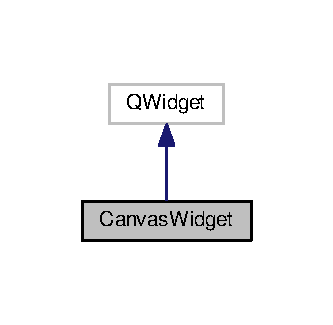
\includegraphics[width=160pt]{classCanvasWidget__inherit__graph}
\end{center}
\end{figure}


Collaboration diagram for Canvas\-Widget\-:\nopagebreak
\begin{figure}[H]
\begin{center}
\leavevmode
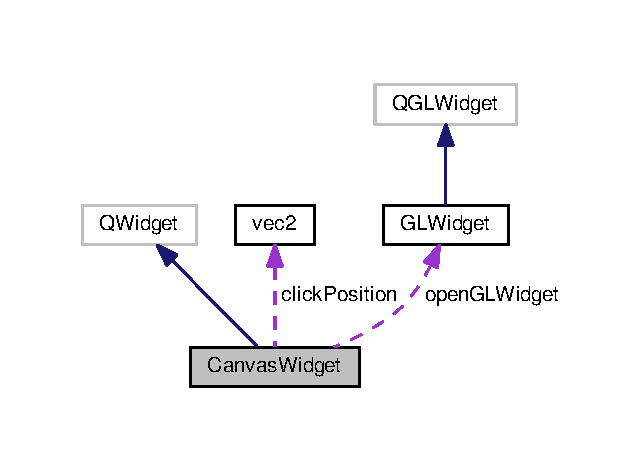
\includegraphics[width=309pt]{classCanvasWidget__coll__graph}
\end{center}
\end{figure}
\subsection*{Public Slots}
\begin{DoxyCompactItemize}
\item 
void \hyperlink{classCanvasWidget_a10d481976a36a4e489f42d2b5dfa4662}{change\-Tool} (int tool)
\item 
\hypertarget{classCanvasWidget_a24a75e8958b478656824d1d985d2d64d}{void {\bfseries open\-Color\-Picker} ()}\label{classCanvasWidget_a24a75e8958b478656824d1d985d2d64d}

\item 
\hypertarget{classCanvasWidget_a3dbc33d4382ea5295af8008760f123f3}{void {\bfseries set\-Current\-Color} (const Q\-Color \&color)}\label{classCanvasWidget_a3dbc33d4382ea5295af8008760f123f3}

\item 
\hypertarget{classCanvasWidget_a6a39b7120018202a7fc095a7638e8c90}{void {\bfseries deselect\-All} ()}\label{classCanvasWidget_a6a39b7120018202a7fc095a7638e8c90}

\item 
\hypertarget{classCanvasWidget_a692ef366f79d844dabc58803a82ba2d4}{void {\bfseries select\-All} ()}\label{classCanvasWidget_a692ef366f79d844dabc58803a82ba2d4}

\item 
\hypertarget{classCanvasWidget_afd4a461b8779e2d692a08647e655bc1e}{void {\bfseries zoom\-In} ()}\label{classCanvasWidget_afd4a461b8779e2d692a08647e655bc1e}

\item 
\hypertarget{classCanvasWidget_a0a19a82e3f4fbe354b779ff014e55ff2}{void {\bfseries zoom\-Out} ()}\label{classCanvasWidget_a0a19a82e3f4fbe354b779ff014e55ff2}

\item 
\hypertarget{classCanvasWidget_a05e567b5107bad5938e32a650c7696a6}{void {\bfseries update\-Size} ()}\label{classCanvasWidget_a05e567b5107bad5938e32a650c7696a6}

\item 
\hypertarget{classCanvasWidget_a9617418393fa64b4d662c0523acd98a2}{void {\bfseries undo} ()}\label{classCanvasWidget_a9617418393fa64b4d662c0523acd98a2}

\item 
\hypertarget{classCanvasWidget_ae6032a56c6be372d9b48fea14dcb1954}{void {\bfseries redo} ()}\label{classCanvasWidget_ae6032a56c6be372d9b48fea14dcb1954}

\item 
\hypertarget{classCanvasWidget_a0ccbb1b2140e5bbadc21ffe0684bd848}{void {\bfseries open} (std\-::string file\-Name)}\label{classCanvasWidget_a0ccbb1b2140e5bbadc21ffe0684bd848}

\item 
\hypertarget{classCanvasWidget_ac7465ba42b77a5a9a36af19073e0279a}{void {\bfseries save\-As} (std\-::string file\-Name)}\label{classCanvasWidget_ac7465ba42b77a5a9a36af19073e0279a}

\end{DoxyCompactItemize}
\subsection*{Signals}
\begin{DoxyCompactItemize}
\item 
\hypertarget{classCanvasWidget_a40301a55d3c5c4af8fdbb9a70942055c}{void {\bfseries color\-Changed} (const Q\-String \&style\-Sheet)}\label{classCanvasWidget_a40301a55d3c5c4af8fdbb9a70942055c}

\item 
\hypertarget{classCanvasWidget_ac2e5cfa7aac9658bf358af1e9b15d99e}{void {\bfseries state\-Changed} ()}\label{classCanvasWidget_ac2e5cfa7aac9658bf358af1e9b15d99e}

\end{DoxyCompactItemize}
\subsection*{Public Member Functions}
\begin{DoxyCompactItemize}
\item 
\hypertarget{classCanvasWidget_a3056d84c95e47f825ab4be09f48c0662}{{\bfseries Canvas\-Widget} (Q\-Widget $\ast$parent=0)}\label{classCanvasWidget_a3056d84c95e47f825ab4be09f48c0662}

\item 
\hypertarget{classCanvasWidget_a990d94414822524b183a4d90330ab13b}{int {\bfseries get\-Current\-Tool} ()}\label{classCanvasWidget_a990d94414822524b183a4d90330ab13b}

\end{DoxyCompactItemize}
\subsection*{Protected Member Functions}
\begin{DoxyCompactItemize}
\item 
\hypertarget{classCanvasWidget_a06806e2eda021c884160067a4148dc32}{void {\bfseries resize\-Event} (Q\-Resize\-Event $\ast$event)}\label{classCanvasWidget_a06806e2eda021c884160067a4148dc32}

\item 
\hypertarget{classCanvasWidget_a635c9e389dcdcc25cf218150b6c8a5cc}{void {\bfseries paint\-Event} (Q\-Paint\-Event $\ast$)}\label{classCanvasWidget_a635c9e389dcdcc25cf218150b6c8a5cc}

\item 
\hypertarget{classCanvasWidget_ab3ec45e42dd3da00012f3fb3e01666d4}{void {\bfseries mouse\-Press\-Event} (Q\-Mouse\-Event $\ast$event)}\label{classCanvasWidget_ab3ec45e42dd3da00012f3fb3e01666d4}

\item 
\hypertarget{classCanvasWidget_aa1ddd11ddeb07b7d4f105bf2959ce9bf}{void {\bfseries mouse\-Release\-Event} (Q\-Mouse\-Event $\ast$event)}\label{classCanvasWidget_aa1ddd11ddeb07b7d4f105bf2959ce9bf}

\item 
\hypertarget{classCanvasWidget_a1f0eced3fa450e2a04239b4fe8e3810a}{void {\bfseries mouse\-Move\-Event} (Q\-Mouse\-Event $\ast$event)}\label{classCanvasWidget_a1f0eced3fa450e2a04239b4fe8e3810a}

\end{DoxyCompactItemize}
\subsection*{Private Member Functions}
\begin{DoxyCompactItemize}
\item 
\hypertarget{classCanvasWidget_a4d553688bfcfc791d640d36587f27c26}{bool {\bfseries event\-Filter} (Q\-Object $\ast$object, Q\-Event $\ast$event)}\label{classCanvasWidget_a4d553688bfcfc791d640d36587f27c26}

\end{DoxyCompactItemize}
\subsection*{Private Attributes}
\begin{DoxyCompactItemize}
\item 
\hypertarget{classCanvasWidget_ad2353cc7b274a6db64eb6229fde95164}{\hyperlink{classGLWidget}{G\-L\-Widget} $\ast$ {\bfseries open\-G\-L\-Widget}}\label{classCanvasWidget_ad2353cc7b274a6db64eb6229fde95164}

\item 
\hypertarget{classCanvasWidget_aa66106798f5355101d44e8c095956cbe}{float {\bfseries zoom}}\label{classCanvasWidget_aa66106798f5355101d44e8c095956cbe}

\item 
\hypertarget{classCanvasWidget_ae3ca83bf96327e9a7ac8f9b85a07a292}{Q\-Color\-Dialog {\bfseries color\-Picker}}\label{classCanvasWidget_ae3ca83bf96327e9a7ac8f9b85a07a292}

\item 
\hypertarget{classCanvasWidget_a4ef50e03625f3d3343ebaabcb6ae93e7}{\hyperlink{classGLWidget_a9fba3eba78950865febd4547be0641d0}{G\-L\-Widget\-::\-Draw\-Tool} {\bfseries current\-Tool}}\label{classCanvasWidget_a4ef50e03625f3d3343ebaabcb6ae93e7}

\item 
\hypertarget{classCanvasWidget_a04b6116842600139d6c67d52dd118fcb}{Q\-Color {\bfseries current\-Color}}\label{classCanvasWidget_a04b6116842600139d6c67d52dd118fcb}

\item 
\hypertarget{classCanvasWidget_aefda1f3eaadbd5788e98f58e572d70b5}{\hyperlink{classvec2}{vec2} {\bfseries click\-Position}}\label{classCanvasWidget_aefda1f3eaadbd5788e98f58e572d70b5}

\item 
\hypertarget{classCanvasWidget_a40257c6897003c90e13cac2e97d644c9}{Q\-Widget $\ast$ {\bfseries main\-Window}}\label{classCanvasWidget_a40257c6897003c90e13cac2e97d644c9}

\item 
\hypertarget{classCanvasWidget_a6370f81145582e8583aca8c65c77be1c}{std\-::string {\bfseries m\-\_\-file\-Name}}\label{classCanvasWidget_a6370f81145582e8583aca8c65c77be1c}

\end{DoxyCompactItemize}


\subsection{Member Function Documentation}
\hypertarget{classCanvasWidget_a10d481976a36a4e489f42d2b5dfa4662}{\index{Canvas\-Widget@{Canvas\-Widget}!change\-Tool@{change\-Tool}}
\index{change\-Tool@{change\-Tool}!CanvasWidget@{Canvas\-Widget}}
\subsubsection[{change\-Tool}]{\setlength{\rightskip}{0pt plus 5cm}void Canvas\-Widget\-::change\-Tool (
\begin{DoxyParamCaption}
\item[{int}]{tool}
\end{DoxyParamCaption}
)\hspace{0.3cm}{\ttfamily [slot]}}}\label{classCanvasWidget_a10d481976a36a4e489f42d2b5dfa4662}
Changes the current tool being used to update the widget. This function calls G\-L\-Widget\-::change\-Tool(int) on the underlying \hyperlink{classGLWidget}{G\-L\-Widget}.


\begin{DoxyParams}{Parameters}
{\em tool} & A \hyperlink{classGLWidget_a9fba3eba78950865febd4547be0641d0}{G\-L\-Widget\-::\-Draw\-Tool} enum that represents the tool the widget should use.\\
\hline
\end{DoxyParams}
\begin{DoxySeeAlso}{See Also}
Canvas\-Widget\-::mouse\-Press\-Event(\-Q\-Event$\ast$) 

Canvas\-Widget\-::mouse\-Move\-Event(\-Q\-Event$\ast$) 

G\-L\-Widget\-::change\-Tool(int) 
\end{DoxySeeAlso}


The documentation for this class was generated from the following files\-:\begin{DoxyCompactItemize}
\item 
src/canvaswidget.\-hpp\item 
src/canvaswidget.\-cpp\end{DoxyCompactItemize}

\hypertarget{classGLWidget}{\section{G\-L\-Widget Class Reference}
\label{classGLWidget}\index{G\-L\-Widget@{G\-L\-Widget}}
}


A Widget for rendering and drawing Bixels.  




{\ttfamily \#include $<$glwidget.\-hpp$>$}



Inheritance diagram for G\-L\-Widget\-:\nopagebreak
\begin{figure}[H]
\begin{center}
\leavevmode
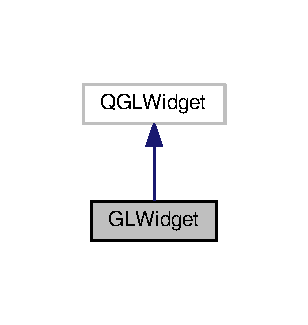
\includegraphics[width=148pt]{classGLWidget__inherit__graph}
\end{center}
\end{figure}


Collaboration diagram for G\-L\-Widget\-:\nopagebreak
\begin{figure}[H]
\begin{center}
\leavevmode
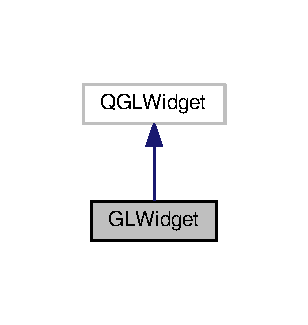
\includegraphics[width=148pt]{classGLWidget__coll__graph}
\end{center}
\end{figure}
\subsection*{Classes}
\begin{DoxyCompactItemize}
\item 
struct \hyperlink{structGLWidget_1_1HistoryState}{History\-State}
\begin{DoxyCompactList}\small\item\em This struct stores the current state of a \hyperlink{classGLWidget}{G\-L\-Widget}. \end{DoxyCompactList}\end{DoxyCompactItemize}
\subsection*{Public Types}
\begin{DoxyCompactItemize}
\item 
enum \hyperlink{classGLWidget_a9fba3eba78950865febd4547be0641d0}{Draw\-Tool} \{ \\*
\hyperlink{classGLWidget_a9fba3eba78950865febd4547be0641d0a53197083abb268d80465c7af0071bfe7}{M\-O\-U\-S\-E}, 
\hyperlink{classGLWidget_a9fba3eba78950865febd4547be0641d0a13dba4ab40790d00786f83a8af372a37}{B\-R\-U\-S\-H}, 
{\bfseries P\-A\-I\-N\-T\-B\-U\-C\-K\-E\-T}, 
\hyperlink{classGLWidget_a9fba3eba78950865febd4547be0641d0a36a243e579dcf431ca1bf5306f9b3459}{E\-R\-A\-S\-E\-R}, 
\\*
\hyperlink{classGLWidget_a9fba3eba78950865febd4547be0641d0ab9c3b71d6caf455913325367c4d00862}{E\-Y\-E\-D\-R\-O\-P}, 
\hyperlink{classGLWidget_a9fba3eba78950865febd4547be0641d0ab807fc933b2f87fde055dd12b61a9ec2}{H\-A\-N\-D}, 
\hyperlink{classGLWidget_a9fba3eba78950865febd4547be0641d0a28331a2b609c88af7845259f23271151}{Z\-O\-O\-M}
 \}
\end{DoxyCompactItemize}
\subsection*{Signals}
\begin{DoxyCompactItemize}
\item 
\hypertarget{classGLWidget_a4a11176bfcdf51d04a18d4383bde7a58}{void {\bfseries state\-Changed} ()}\label{classGLWidget_a4a11176bfcdf51d04a18d4383bde7a58}

\end{DoxyCompactItemize}
\subsection*{Public Member Functions}
\begin{DoxyCompactItemize}
\item 
\hyperlink{classGLWidget_ab79c391c86de1ffb76f6950b49d82c0c}{G\-L\-Widget} (Q\-Widget $\ast$parent=0)
\begin{DoxyCompactList}\small\item\em Initializes the \hyperlink{classGLWidget}{G\-L\-Widget} with a parent widget. \end{DoxyCompactList}\item 
void \hyperlink{classGLWidget_a6e0dab354b3abec59774c29f82346ebe}{draw\-Square} (Q\-Color color, \hyperlink{classvec2}{vec2} position, double size, bool outline\-Only=false)
\item 
bool \hyperlink{classGLWidget_aebdd7462523ecff734ac224031ec9e0b}{save\-File} (const std\-::string \&file\-Name)
\begin{DoxyCompactList}\small\item\em This will save a file {\ttfamily file\-Name} using Q\-Data\-Stream version (Qt 4.\-9). \end{DoxyCompactList}\item 
bool \hyperlink{classGLWidget_a7c2c4eee95553aad627843b865d3bc23}{open\-File} (const std\-::string \&file\-Name)
\begin{DoxyCompactList}\small\item\em This will load a file {\ttfamily file\-Name} using Q\-Data\-Stream version (Qt 4.\-9). \end{DoxyCompactList}\item 
void \hyperlink{classGLWidget_a603764586aa51ed3fbdd06ac9c658e6b}{increase\-Dimension} ()
\begin{DoxyCompactList}\small\item\em This will multiply the \hyperlink{classGLWidget_a0ecdf8ea93e62ab9d294714e59dafd64}{dimension} of the widget by 2. \end{DoxyCompactList}\item 
void \hyperlink{classGLWidget_a34c77d5e886569ec84123bb0da5a0751}{decrease\-Dimension} ()
\item 
void \hyperlink{classGLWidget_aed44b9ce42449cf8f086a743bbbac7cd}{undo} ()
\begin{DoxyCompactList}\small\item\em An implementation of the undo function. \end{DoxyCompactList}\item 
void \hyperlink{classGLWidget_a5371a80ec723e710374f302611710e15}{redo} ()
\begin{DoxyCompactList}\small\item\em An implementation of redo. \end{DoxyCompactList}\end{DoxyCompactItemize}
\begin{Indent}{\bf Public Bixel Selectors}\par
{\em These are all methods that add or remove Bixels from \hyperlink{classGLWidget_ab07a9ee710f42da54d0158cbdedf3674}{selected\-Bixels}. }\begin{DoxyCompactItemize}
\item 
void \hyperlink{classGLWidget_a1acd74645ffbe6bc071365c2bbd176ba}{fill\-Selected} ()
\item 
void \hyperlink{classGLWidget_ac41fdd4181036c79f4bdf688045155b3}{select\-Bixel\-At} (int i, int j)
\item 
\hypertarget{classGLWidget_a75bca3161b8929b5190fa066cc14cc21}{void {\bfseries select\-Bixel\-At} (Color\-Matrix\-Index i)}\label{classGLWidget_a75bca3161b8929b5190fa066cc14cc21}

\item 
void \hyperlink{classGLWidget_a9ecf9af9846dacfa9cbf17cecc478145}{deselect\-Bixel\-At} (int i, int j)
\item 
void \hyperlink{classGLWidget_aa17c9adb76b61f1f0c4a285f538ce80d}{deselect\-All} ()
\item 
void \hyperlink{classGLWidget_abe918fd89a3f4c4f3d8864efee282610}{select\-All} ()
\item 
void \hyperlink{classGLWidget_a0f0089107cb0fbe89b337dfc01384e28}{select\-Rectangle} (const std\-::vector$<$ int $>$ \&p1, const std\-::vector$<$ int $>$ \&p2)
\end{DoxyCompactItemize}
\end{Indent}
\begin{Indent}{\bf Public Access Methods}\par
\begin{DoxyCompactItemize}
\item 
Q\-Color \hyperlink{classGLWidget_ab67274be71693397e33bcb5f644e8d6a}{get\-Color\-At} (int i, int j)
\item 
\hyperlink{classGLWidget_a9fba3eba78950865febd4547be0641d0}{Draw\-Tool} \hyperlink{classGLWidget_ad7b5ee8248e47c8c1c9c1525c9e5acce}{tool} ()
\item 
int \hyperlink{classGLWidget_a0ecdf8ea93e62ab9d294714e59dafd64}{dimension} ()
\begin{DoxyCompactList}\small\item\em The dimension of the \hyperlink{classGLWidget}{G\-L\-Widget} is the smallest of \hyperlink{classGLWidget_a272046b9cb9f26f5b382f9a121672570}{grid\-Width} and \hyperlink{classGLWidget_a419c32eef067d7157b00904dd52bdb8b}{grid\-Height}. \end{DoxyCompactList}\item 
int \hyperlink{classGLWidget_a272046b9cb9f26f5b382f9a121672570}{grid\-Width} ()
\item 
int \hyperlink{classGLWidget_a419c32eef067d7157b00904dd52bdb8b}{grid\-Height} ()
\item 
Q\-Color \hyperlink{classGLWidget_a8ea9c1e6b1013897e22dc7121f377113}{drawing\-Color} ()
\item 
std\-::vector$<$ Q\-Color $>$ \hyperlink{classGLWidget_aab1b8762be4b33d384e3689427c2addc}{color\-Matrix} ()
\item 
std\-::set$<$ Color\-Matrix\-Index $>$ \hyperlink{classGLWidget_ab07a9ee710f42da54d0158cbdedf3674}{selected\-Bixels} ()
\end{DoxyCompactItemize}
\end{Indent}
\begin{Indent}{\bf Public Mutator Methods}\par
\begin{DoxyCompactItemize}
\item 
void \hyperlink{classGLWidget_ab712fb8b0f65e689a21749062bd2f8d7}{change\-Tool} (\hyperlink{classGLWidget_a9fba3eba78950865febd4547be0641d0}{Draw\-Tool} \hyperlink{classGLWidget_ad7b5ee8248e47c8c1c9c1525c9e5acce}{tool})
\item 
void \hyperlink{classGLWidget_a5abf53a0389c884788c3c106a7a1263d}{set\-Color\-At} (int i, int j, Q\-Color color)
\item 
\hypertarget{classGLWidget_a94d23dd2ecad4f803fee7eb82a6bb4d3}{void {\bfseries set\-Color\-At} (Color\-Matrix\-Index i, Q\-Color color)}\label{classGLWidget_a94d23dd2ecad4f803fee7eb82a6bb4d3}

\item 
void \hyperlink{classGLWidget_a087325630069166821ada20445fc89a6}{set\-Drawing\-Color} (const Q\-Color \&color)
\end{DoxyCompactItemize}
\end{Indent}
\subsection*{Protected Member Functions}
\begin{DoxyCompactItemize}
\item 
void \hyperlink{classGLWidget_a7fab13e8cc9fc0730ca54c08b2c923a7}{initialize\-G\-L} ()
\item 
void \hyperlink{classGLWidget_a640b5570cb2b37724fd5b58a77339c5e}{paint\-G\-L} ()
\item 
void \hyperlink{classGLWidget_ac0d2a8ecf60907a81c0d73475d851025}{resize\-G\-L} (int width, int height)
\item 
void \hyperlink{classGLWidget_ab144cc8064c1bbf6d0ef0646ca0bd06c}{mouse\-Press\-Event} (Q\-Mouse\-Event $\ast$event)
\item 
void \hyperlink{classGLWidget_a9043bac13d6f0a5307ea5c7f9b3caa50}{mouse\-Move\-Event} (Q\-Mouse\-Event $\ast$event)
\item 
void \hyperlink{classGLWidget_ab992c4c25439a5ef23031991015451c1}{mouse\-Release\-Event} (Q\-Mouse\-Event $\ast$event)
\begin{DoxyCompactList}\small\item\em Called whenever the mouse is released. \end{DoxyCompactList}\item 
void \hyperlink{classGLWidget_a43dfdc9164dfacb939a173e725651fa9}{key\-Press\-Event} (Q\-Key\-Event $\ast$event)
\begin{DoxyCompactList}\small\item\em Called whenever a Key is pressed. \end{DoxyCompactList}\item 
void \hyperlink{classGLWidget_a3fff7f887bf2ab1df58c870fb6146f31}{key\-Release\-Event} (Q\-Key\-Event $\ast$)
\item 
void \hyperlink{classGLWidget_a9c9e2bd40c564a1e6a4df98960355b6e}{save\-History\-State} ()
\begin{DoxyCompactList}\small\item\em Saves the current state of the \hyperlink{classGLWidget}{G\-L\-Widget}. \end{DoxyCompactList}\item 
bool \hyperlink{classGLWidget_acb2ac0440f3e004a77c31f8b035fb8a4}{load\-History\-State} (int state\-Index)
\item 
Color\-Matrix\-Index \hyperlink{classGLWidget_a6d19cf2624d93499c40163ddb4091783}{color\-Matrix\-Index} (int i, int j) const 
\item 
\hyperlink{classvec2}{vec2} \hyperlink{classGLWidget_ab464e7edbe7729a853d7ccb510d6ef73}{normalize\-Coordinates} (\hyperlink{classvec2}{vec2} coord) const 
\end{DoxyCompactItemize}
\subsection*{Private Types}
\begin{DoxyCompactItemize}
\item 
\hypertarget{classGLWidget_a5a2947849a31320f39477d93511712e5}{typedef int {\bfseries Color\-Matrix\-Index}}\label{classGLWidget_a5a2947849a31320f39477d93511712e5}

\end{DoxyCompactItemize}
\subsection*{Private Member Functions}
\begin{DoxyCompactItemize}
\item 
std\-::vector$<$ int $>$ \hyperlink{classGLWidget_a7555011afa685031ca05eaebe7d673cc}{convert\-Position\-To\-Bixel\-Index} (int x, int y) const 
\item 
float \hyperlink{classGLWidget_a9e1d6025155e0e95331f3dd8a8a4db62}{calculate\-Bixel\-Width} ()
\end{DoxyCompactItemize}


\subsection{Detailed Description}
A Widget for rendering and drawing Bixels. 

\begin{DoxyRefDesc}{What I am currently doing}
\item[\hyperlink{task__task000001}{What I am currently doing}]Adding a m\-\_\-marked\-Bixels vector that will contain every Bixel that has been changed since the last call to \hyperlink{classGLWidget_a640b5570cb2b37724fd5b58a77339c5e}{paint\-G\-L}.
\begin{DoxyItemize}
\item Create the member variable $\ast$$\ast$$\ast$
\item Create a mark\-Bixel(int i, int j) method
\item Go through every mutator of \hyperlink{classGLWidget_aab1b8762be4b33d384e3689427c2addc}{color\-Matrix} and add a call to mark\-Bixel(int i, int j)
\item Update paint\-G\-L to draw only the bixels that have been marked. 
\end{DoxyItemize}\end{DoxyRefDesc}
The \hyperlink{classGLWidget}{G\-L\-Widget} is used as the canvas for the user to draw and edit .bixl files using various tools. The Widget is defined by a grid of width \hyperlink{classGLWidget_a272046b9cb9f26f5b382f9a121672570}{grid\-Width} and height \hyperlink{classGLWidget_a419c32eef067d7157b00904dd52bdb8b}{grid\-Height}.

\begin{DoxySeeAlso}{See Also}
\hyperlink{classCanvasWidget}{Canvas\-Widget} 
\end{DoxySeeAlso}
\begin{DoxyRefDesc}{High Priority Todo}
\item[\hyperlink{todo1__todo1000001}{High Priority Todo}]Make sure delicate members like m\-\_\-color\-Matrix and m\-\_\-selected\-Bixels are only accessed through accessor and mutator methods. \end{DoxyRefDesc}
\begin{DoxyRefDesc}{Todo}
\item[\hyperlink{todo__todo000010}{Todo}]Rename to Bixel\-Grid or something \end{DoxyRefDesc}


\subsection{Member Enumeration Documentation}
\hypertarget{classGLWidget_a9fba3eba78950865febd4547be0641d0}{\index{G\-L\-Widget@{G\-L\-Widget}!Draw\-Tool@{Draw\-Tool}}
\index{Draw\-Tool@{Draw\-Tool}!GLWidget@{G\-L\-Widget}}
\subsubsection[{Draw\-Tool}]{\setlength{\rightskip}{0pt plus 5cm}enum {\bf G\-L\-Widget\-::\-Draw\-Tool}}}\label{classGLWidget_a9fba3eba78950865febd4547be0641d0}
Represents the tools in the toolbar \begin{DoxySeeAlso}{See Also}
\hyperlink{classCanvasWidget_a10d481976a36a4e489f42d2b5dfa4662}{Canvas\-Widget\-::change\-Tool(int)} 

G\-L\-Widget\-::change\-Tool(int) 
\end{DoxySeeAlso}
\begin{DoxyRefDesc}{Todo}
\item[\hyperlink{todo__todo000011}{Todo}]Move H\-A\-N\-D and Z\-O\-O\-M to an enum in \hyperlink{classCanvasWidget}{Canvas\-Widget}. 

Implement E\-Y\-E\-D\-R\-O\-P 

Add a Paint\-Bucket tool. 

Add a Magic wand tool. 

Flesh out tools enum documentation \end{DoxyRefDesc}
\begin{Desc}
\item[Enumerator]\par
\begin{description}
\index{M\-O\-U\-S\-E@{M\-O\-U\-S\-E}!G\-L\-Widget@{G\-L\-Widget}}\index{G\-L\-Widget@{G\-L\-Widget}!M\-O\-U\-S\-E@{M\-O\-U\-S\-E}}\item[{\em 
\hypertarget{classGLWidget_a9fba3eba78950865febd4547be0641d0a53197083abb268d80465c7af0071bfe7}{M\-O\-U\-S\-E}\label{classGLWidget_a9fba3eba78950865febd4547be0641d0a53197083abb268d80465c7af0071bfe7}
}]Used to select Bixels. \index{B\-R\-U\-S\-H@{B\-R\-U\-S\-H}!G\-L\-Widget@{G\-L\-Widget}}\index{G\-L\-Widget@{G\-L\-Widget}!B\-R\-U\-S\-H@{B\-R\-U\-S\-H}}\item[{\em 
\hypertarget{classGLWidget_a9fba3eba78950865febd4547be0641d0a13dba4ab40790d00786f83a8af372a37}{B\-R\-U\-S\-H}\label{classGLWidget_a9fba3eba78950865febd4547be0641d0a13dba4ab40790d00786f83a8af372a37}
}]Used to Color Bixels. \index{E\-R\-A\-S\-E\-R@{E\-R\-A\-S\-E\-R}!G\-L\-Widget@{G\-L\-Widget}}\index{G\-L\-Widget@{G\-L\-Widget}!E\-R\-A\-S\-E\-R@{E\-R\-A\-S\-E\-R}}\item[{\em 
\hypertarget{classGLWidget_a9fba3eba78950865febd4547be0641d0a36a243e579dcf431ca1bf5306f9b3459}{E\-R\-A\-S\-E\-R}\label{classGLWidget_a9fba3eba78950865febd4547be0641d0a36a243e579dcf431ca1bf5306f9b3459}
}]Used to set Bixel color to (0, 0, 0, 0) \index{E\-Y\-E\-D\-R\-O\-P@{E\-Y\-E\-D\-R\-O\-P}!G\-L\-Widget@{G\-L\-Widget}}\index{G\-L\-Widget@{G\-L\-Widget}!E\-Y\-E\-D\-R\-O\-P@{E\-Y\-E\-D\-R\-O\-P}}\item[{\em 
\hypertarget{classGLWidget_a9fba3eba78950865febd4547be0641d0ab9c3b71d6caf455913325367c4d00862}{E\-Y\-E\-D\-R\-O\-P}\label{classGLWidget_a9fba3eba78950865febd4547be0641d0ab9c3b71d6caf455913325367c4d00862}
}]The Eyedrop Tool. \index{H\-A\-N\-D@{H\-A\-N\-D}!G\-L\-Widget@{G\-L\-Widget}}\index{G\-L\-Widget@{G\-L\-Widget}!H\-A\-N\-D@{H\-A\-N\-D}}\item[{\em 
\hypertarget{classGLWidget_a9fba3eba78950865febd4547be0641d0ab807fc933b2f87fde055dd12b61a9ec2}{H\-A\-N\-D}\label{classGLWidget_a9fba3eba78950865febd4547be0641d0ab807fc933b2f87fde055dd12b61a9ec2}
}]The Hand Tool. \index{Z\-O\-O\-M@{Z\-O\-O\-M}!G\-L\-Widget@{G\-L\-Widget}}\index{G\-L\-Widget@{G\-L\-Widget}!Z\-O\-O\-M@{Z\-O\-O\-M}}\item[{\em 
\hypertarget{classGLWidget_a9fba3eba78950865febd4547be0641d0a28331a2b609c88af7845259f23271151}{Z\-O\-O\-M}\label{classGLWidget_a9fba3eba78950865febd4547be0641d0a28331a2b609c88af7845259f23271151}
}]The Zoom Tool. \end{description}
\end{Desc}


\subsection{Constructor \& Destructor Documentation}
\hypertarget{classGLWidget_ab79c391c86de1ffb76f6950b49d82c0c}{\index{G\-L\-Widget@{G\-L\-Widget}!G\-L\-Widget@{G\-L\-Widget}}
\index{G\-L\-Widget@{G\-L\-Widget}!GLWidget@{G\-L\-Widget}}
\subsubsection[{G\-L\-Widget}]{\setlength{\rightskip}{0pt plus 5cm}G\-L\-Widget\-::\-G\-L\-Widget (
\begin{DoxyParamCaption}
\item[{Q\-Widget $\ast$}]{parent = {\ttfamily 0}}
\end{DoxyParamCaption}
)}}\label{classGLWidget_ab79c391c86de1ffb76f6950b49d82c0c}


Initializes the \hyperlink{classGLWidget}{G\-L\-Widget} with a parent widget. 

The constructor initializes all private fields. It then calls \hyperlink{classGLWidget_a9c9e2bd40c564a1e6a4df98960355b6e}{save\-History\-State}, Q\-Widget\-::set\-Focus, and Q\-Widget\-::set\-Focus\-Policy(\-Qt\-::\-Strong\-Focus).


\begin{DoxyParams}{Parameters}
{\em parent} & The parent Q\-Widget. \\
\hline
\end{DoxyParams}


\subsection{Member Function Documentation}
\hypertarget{classGLWidget_a9e1d6025155e0e95331f3dd8a8a4db62}{\index{G\-L\-Widget@{G\-L\-Widget}!calculate\-Bixel\-Width@{calculate\-Bixel\-Width}}
\index{calculate\-Bixel\-Width@{calculate\-Bixel\-Width}!GLWidget@{G\-L\-Widget}}
\subsubsection[{calculate\-Bixel\-Width}]{\setlength{\rightskip}{0pt plus 5cm}float G\-L\-Widget\-::calculate\-Bixel\-Width (
\begin{DoxyParamCaption}
{}
\end{DoxyParamCaption}
)\hspace{0.3cm}{\ttfamily [private]}}}\label{classGLWidget_a9e1d6025155e0e95331f3dd8a8a4db62}
Returns the width of one cell in \hyperlink{classGLWidget_aab1b8762be4b33d384e3689427c2addc}{color\-Matrix} relative to \hyperlink{classGLWidget}{G\-L\-Widget}. \hypertarget{classGLWidget_ab712fb8b0f65e689a21749062bd2f8d7}{\index{G\-L\-Widget@{G\-L\-Widget}!change\-Tool@{change\-Tool}}
\index{change\-Tool@{change\-Tool}!GLWidget@{G\-L\-Widget}}
\subsubsection[{change\-Tool}]{\setlength{\rightskip}{0pt plus 5cm}void G\-L\-Widget\-::change\-Tool (
\begin{DoxyParamCaption}
\item[{{\bf G\-L\-Widget\-::\-Draw\-Tool}}]{tool}
\end{DoxyParamCaption}
)}}\label{classGLWidget_ab712fb8b0f65e689a21749062bd2f8d7}
Changes the current tool being used to update the widget.

\begin{DoxySeeAlso}{See Also}
G\-L\-Widget\-::mouse\-Press\-Event(\-Q\-Event$\ast$) 

G\-L\-Widget\-::mouse\-Move\-Event(\-Q\-Event$\ast$) 
\end{DoxySeeAlso}
\hypertarget{classGLWidget_aab1b8762be4b33d384e3689427c2addc}{\index{G\-L\-Widget@{G\-L\-Widget}!color\-Matrix@{color\-Matrix}}
\index{color\-Matrix@{color\-Matrix}!GLWidget@{G\-L\-Widget}}
\subsubsection[{color\-Matrix}]{\setlength{\rightskip}{0pt plus 5cm}std\-::vector$<$ Q\-Color $>$ G\-L\-Widget\-::color\-Matrix (
\begin{DoxyParamCaption}
{}
\end{DoxyParamCaption}
)}}\label{classGLWidget_aab1b8762be4b33d384e3689427c2addc}
This returns the main color\-Matrix as a 2d vector. \begin{DoxyRefDesc}{Todo}
\item[\hyperlink{todo__todo000001}{Todo}]Copy m\-\_\-color\-Matrix into a 2d vector and return that instead of the raw color\-Matrix. 

Maybe create setters for color\-Matrix. \end{DoxyRefDesc}
\hypertarget{classGLWidget_a6d19cf2624d93499c40163ddb4091783}{\index{G\-L\-Widget@{G\-L\-Widget}!color\-Matrix\-Index@{color\-Matrix\-Index}}
\index{color\-Matrix\-Index@{color\-Matrix\-Index}!GLWidget@{G\-L\-Widget}}
\subsubsection[{color\-Matrix\-Index}]{\setlength{\rightskip}{0pt plus 5cm}G\-L\-Widget\-::\-Color\-Matrix\-Index G\-L\-Widget\-::color\-Matrix\-Index (
\begin{DoxyParamCaption}
\item[{int}]{i, }
\item[{int}]{j}
\end{DoxyParamCaption}
) const\hspace{0.3cm}{\ttfamily [protected]}}}\label{classGLWidget_a6d19cf2624d93499c40163ddb4091783}
Converts a 2d matrix index to a vector index to be used with \hyperlink{classGLWidget_aab1b8762be4b33d384e3689427c2addc}{color\-Matrix}.

\begin{DoxyReturn}{Returns}
A Color\-Matrix\-Index int to be used when accessing an element of \hyperlink{classGLWidget_aab1b8762be4b33d384e3689427c2addc}{color\-Matrix} directly, or searching \hyperlink{classGLWidget_ab07a9ee710f42da54d0158cbdedf3674}{selected\-Bixels}. 
\end{DoxyReturn}
\hypertarget{classGLWidget_a7555011afa685031ca05eaebe7d673cc}{\index{G\-L\-Widget@{G\-L\-Widget}!convert\-Position\-To\-Bixel\-Index@{convert\-Position\-To\-Bixel\-Index}}
\index{convert\-Position\-To\-Bixel\-Index@{convert\-Position\-To\-Bixel\-Index}!GLWidget@{G\-L\-Widget}}
\subsubsection[{convert\-Position\-To\-Bixel\-Index}]{\setlength{\rightskip}{0pt plus 5cm}std\-::vector$<$ int $>$ G\-L\-Widget\-::convert\-Position\-To\-Bixel\-Index (
\begin{DoxyParamCaption}
\item[{int}]{x, }
\item[{int}]{y}
\end{DoxyParamCaption}
) const\hspace{0.3cm}{\ttfamily [private]}}}\label{classGLWidget_a7555011afa685031ca05eaebe7d673cc}
Converts a position relative to the Widget to an index of \hyperlink{classGLWidget_aab1b8762be4b33d384e3689427c2addc}{color\-Matrix}.

\begin{DoxyReturn}{Returns}
A vector of the form $<$i, j$>$ 
\end{DoxyReturn}
\hypertarget{classGLWidget_a34c77d5e886569ec84123bb0da5a0751}{\index{G\-L\-Widget@{G\-L\-Widget}!decrease\-Dimension@{decrease\-Dimension}}
\index{decrease\-Dimension@{decrease\-Dimension}!GLWidget@{G\-L\-Widget}}
\subsubsection[{decrease\-Dimension}]{\setlength{\rightskip}{0pt plus 5cm}void G\-L\-Widget\-::decrease\-Dimension (
\begin{DoxyParamCaption}
{}
\end{DoxyParamCaption}
)}}\label{classGLWidget_a34c77d5e886569ec84123bb0da5a0751}
\begin{DoxyRefDesc}{Todo}
\item[\hyperlink{todo__todo000004}{Todo}]Get rid of this. See the todos in \hyperlink{classGLWidget_a603764586aa51ed3fbdd06ac9c658e6b}{increase\-Dimension}. \end{DoxyRefDesc}
\hypertarget{classGLWidget_aa17c9adb76b61f1f0c4a285f538ce80d}{\index{G\-L\-Widget@{G\-L\-Widget}!deselect\-All@{deselect\-All}}
\index{deselect\-All@{deselect\-All}!GLWidget@{G\-L\-Widget}}
\subsubsection[{deselect\-All}]{\setlength{\rightskip}{0pt plus 5cm}void G\-L\-Widget\-::deselect\-All (
\begin{DoxyParamCaption}
{}
\end{DoxyParamCaption}
)}}\label{classGLWidget_aa17c9adb76b61f1f0c4a285f538ce80d}
This will clear the set of Bixels in \hyperlink{classGLWidget_ab07a9ee710f42da54d0158cbdedf3674}{selected\-Bixels}. It will also call \hyperlink{classGLWidget_a640b5570cb2b37724fd5b58a77339c5e}{paint\-G\-L}. \hypertarget{classGLWidget_a9ecf9af9846dacfa9cbf17cecc478145}{\index{G\-L\-Widget@{G\-L\-Widget}!deselect\-Bixel\-At@{deselect\-Bixel\-At}}
\index{deselect\-Bixel\-At@{deselect\-Bixel\-At}!GLWidget@{G\-L\-Widget}}
\subsubsection[{deselect\-Bixel\-At}]{\setlength{\rightskip}{0pt plus 5cm}void G\-L\-Widget\-::deselect\-Bixel\-At (
\begin{DoxyParamCaption}
\item[{int}]{i, }
\item[{int}]{j}
\end{DoxyParamCaption}
)}}\label{classGLWidget_a9ecf9af9846dacfa9cbf17cecc478145}
This will remove a Bixel index ({\ttfamily i}, {\ttfamily j}) from \hyperlink{classGLWidget_ab07a9ee710f42da54d0158cbdedf3674}{selected\-Bixels} if it is already selected. \hypertarget{classGLWidget_a0ecdf8ea93e62ab9d294714e59dafd64}{\index{G\-L\-Widget@{G\-L\-Widget}!dimension@{dimension}}
\index{dimension@{dimension}!GLWidget@{G\-L\-Widget}}
\subsubsection[{dimension}]{\setlength{\rightskip}{0pt plus 5cm}int G\-L\-Widget\-::dimension (
\begin{DoxyParamCaption}
{}
\end{DoxyParamCaption}
)}}\label{classGLWidget_a0ecdf8ea93e62ab9d294714e59dafd64}


The dimension of the \hyperlink{classGLWidget}{G\-L\-Widget} is the smallest of \hyperlink{classGLWidget_a272046b9cb9f26f5b382f9a121672570}{grid\-Width} and \hyperlink{classGLWidget_a419c32eef067d7157b00904dd52bdb8b}{grid\-Height}. 

\begin{DoxyRefDesc}{Todo}
\item[\hyperlink{todo__todo000002}{Todo}]Get rid of this. See \hyperlink{classGLWidget_a603764586aa51ed3fbdd06ac9c658e6b}{increase\-Dimension} todos. \end{DoxyRefDesc}
\hypertarget{classGLWidget_a8ea9c1e6b1013897e22dc7121f377113}{\index{G\-L\-Widget@{G\-L\-Widget}!drawing\-Color@{drawing\-Color}}
\index{drawing\-Color@{drawing\-Color}!GLWidget@{G\-L\-Widget}}
\subsubsection[{drawing\-Color}]{\setlength{\rightskip}{0pt plus 5cm}Q\-Color G\-L\-Widget\-::drawing\-Color (
\begin{DoxyParamCaption}
{}
\end{DoxyParamCaption}
)}}\label{classGLWidget_a8ea9c1e6b1013897e22dc7121f377113}
This is the current color used by the B\-R\-U\-S\-H tool. \hypertarget{classGLWidget_a6e0dab354b3abec59774c29f82346ebe}{\index{G\-L\-Widget@{G\-L\-Widget}!draw\-Square@{draw\-Square}}
\index{draw\-Square@{draw\-Square}!GLWidget@{G\-L\-Widget}}
\subsubsection[{draw\-Square}]{\setlength{\rightskip}{0pt plus 5cm}void G\-L\-Widget\-::draw\-Square (
\begin{DoxyParamCaption}
\item[{Q\-Color}]{color, }
\item[{{\bf vec2}}]{position, }
\item[{double}]{size, }
\item[{bool}]{outline\-Only = {\ttfamily false}}
\end{DoxyParamCaption}
)}}\label{classGLWidget_a6e0dab354b3abec59774c29f82346ebe}
This method draws a square using square\-Shader.\-vert and square\-Shader.\-frag.


\begin{DoxyParams}{Parameters}
{\em color} & The rgba color of the square.\\
\hline
{\em position} & This attribute specifies the bottom left corner of the square. It should be a position relative to the Widget as it will be normalized for Open\-G\-L.\\
\hline
{\em outline\-Only} & If true, G\-L\-\_\-\-L\-I\-N\-E\-\_\-\-L\-O\-O\-P will be used to draw only the outline of the square. \\
\hline
\end{DoxyParams}
\hypertarget{classGLWidget_a1acd74645ffbe6bc071365c2bbd176ba}{\index{G\-L\-Widget@{G\-L\-Widget}!fill\-Selected@{fill\-Selected}}
\index{fill\-Selected@{fill\-Selected}!GLWidget@{G\-L\-Widget}}
\subsubsection[{fill\-Selected}]{\setlength{\rightskip}{0pt plus 5cm}void G\-L\-Widget\-::fill\-Selected (
\begin{DoxyParamCaption}
{}
\end{DoxyParamCaption}
)}}\label{classGLWidget_a1acd74645ffbe6bc071365c2bbd176ba}
This will change the color in \hyperlink{classGLWidget_aab1b8762be4b33d384e3689427c2addc}{color\-Matrix} of all of the Bixels in \hyperlink{classGLWidget_ab07a9ee710f42da54d0158cbdedf3674}{selected\-Bixels} to \hyperlink{classGLWidget_a8ea9c1e6b1013897e22dc7121f377113}{drawing\-Color}. \hypertarget{classGLWidget_ab67274be71693397e33bcb5f644e8d6a}{\index{G\-L\-Widget@{G\-L\-Widget}!get\-Color\-At@{get\-Color\-At}}
\index{get\-Color\-At@{get\-Color\-At}!GLWidget@{G\-L\-Widget}}
\subsubsection[{get\-Color\-At}]{\setlength{\rightskip}{0pt plus 5cm}Q\-Color G\-L\-Widget\-::get\-Color\-At (
\begin{DoxyParamCaption}
\item[{int}]{i, }
\item[{int}]{j}
\end{DoxyParamCaption}
)}}\label{classGLWidget_ab67274be71693397e33bcb5f644e8d6a}
This returns the color of the Bixel in \hyperlink{classGLWidget_aab1b8762be4b33d384e3689427c2addc}{color\-Matrix} at {\ttfamily i} and {\ttfamily j}.


\begin{DoxyParams}{Parameters}
{\em i} & The number of Bixels from the left of the Bixel Grid. \\
\hline
{\em j} & The number of Bixels from the {\bfseries bottom} of the Bixel Grid. \\
\hline
\end{DoxyParams}
\hypertarget{classGLWidget_a419c32eef067d7157b00904dd52bdb8b}{\index{G\-L\-Widget@{G\-L\-Widget}!grid\-Height@{grid\-Height}}
\index{grid\-Height@{grid\-Height}!GLWidget@{G\-L\-Widget}}
\subsubsection[{grid\-Height}]{\setlength{\rightskip}{0pt plus 5cm}int G\-L\-Widget\-::grid\-Height (
\begin{DoxyParamCaption}
{}
\end{DoxyParamCaption}
)}}\label{classGLWidget_a419c32eef067d7157b00904dd52bdb8b}
This is the current height of the grid containing the Bixels. This will always be a multiple of 2. \hypertarget{classGLWidget_a272046b9cb9f26f5b382f9a121672570}{\index{G\-L\-Widget@{G\-L\-Widget}!grid\-Width@{grid\-Width}}
\index{grid\-Width@{grid\-Width}!GLWidget@{G\-L\-Widget}}
\subsubsection[{grid\-Width}]{\setlength{\rightskip}{0pt plus 5cm}int G\-L\-Widget\-::grid\-Width (
\begin{DoxyParamCaption}
{}
\end{DoxyParamCaption}
)}}\label{classGLWidget_a272046b9cb9f26f5b382f9a121672570}
This is the current width of the grid containing the Bixels. This will always be a multiple of 2. \hypertarget{classGLWidget_a603764586aa51ed3fbdd06ac9c658e6b}{\index{G\-L\-Widget@{G\-L\-Widget}!increase\-Dimension@{increase\-Dimension}}
\index{increase\-Dimension@{increase\-Dimension}!GLWidget@{G\-L\-Widget}}
\subsubsection[{increase\-Dimension}]{\setlength{\rightskip}{0pt plus 5cm}void G\-L\-Widget\-::increase\-Dimension (
\begin{DoxyParamCaption}
{}
\end{DoxyParamCaption}
)}}\label{classGLWidget_a603764586aa51ed3fbdd06ac9c658e6b}


This will multiply the \hyperlink{classGLWidget_a0ecdf8ea93e62ab9d294714e59dafd64}{dimension} of the widget by 2. 

This will also update the \hyperlink{classGLWidget_a272046b9cb9f26f5b382f9a121672570}{grid\-Width} and the \hyperlink{classGLWidget_a419c32eef067d7157b00904dd52bdb8b}{grid\-Height}.

\begin{DoxyRefDesc}{Todo}
\item[\hyperlink{todo__todo000003}{Todo}]The way I have been dealing with \hyperlink{classGLWidget_a0ecdf8ea93e62ab9d294714e59dafd64}{dimension} is ridiculous. Get rid of m\-\_\-dimension altogether and use only \hyperlink{classGLWidget_a272046b9cb9f26f5b382f9a121672570}{grid\-Width} and \hyperlink{classGLWidget_a419c32eef067d7157b00904dd52bdb8b}{grid\-Height}. Create an increase\-Width() and an increase\-Height() as well as a decrease\-Width/\-Height. \end{DoxyRefDesc}
\hypertarget{classGLWidget_a7fab13e8cc9fc0730ca54c08b2c923a7}{\index{G\-L\-Widget@{G\-L\-Widget}!initialize\-G\-L@{initialize\-G\-L}}
\index{initialize\-G\-L@{initialize\-G\-L}!GLWidget@{G\-L\-Widget}}
\subsubsection[{initialize\-G\-L}]{\setlength{\rightskip}{0pt plus 5cm}void G\-L\-Widget\-::initialize\-G\-L (
\begin{DoxyParamCaption}
{}
\end{DoxyParamCaption}
)\hspace{0.3cm}{\ttfamily [protected]}}}\label{classGLWidget_a7fab13e8cc9fc0730ca54c08b2c923a7}
\begin{DoxyRefDesc}{Todo}
\item[\hyperlink{todo__todo000006}{Todo}]Make this private. \end{DoxyRefDesc}
\hypertarget{classGLWidget_a43dfdc9164dfacb939a173e725651fa9}{\index{G\-L\-Widget@{G\-L\-Widget}!key\-Press\-Event@{key\-Press\-Event}}
\index{key\-Press\-Event@{key\-Press\-Event}!GLWidget@{G\-L\-Widget}}
\subsubsection[{key\-Press\-Event}]{\setlength{\rightskip}{0pt plus 5cm}void G\-L\-Widget\-::key\-Press\-Event (
\begin{DoxyParamCaption}
\item[{Q\-Key\-Event $\ast$}]{event}
\end{DoxyParamCaption}
)\hspace{0.3cm}{\ttfamily [protected]}}}\label{classGLWidget_a43dfdc9164dfacb939a173e725651fa9}


Called whenever a Key is pressed. 

This method contains method calls depending on the Key pressed.


\begin{DoxyItemize}
\item {\bfseries Backspace}\-: Erases selected Bixels
\item {\bfseries Return}\-: \hyperlink{classGLWidget_a1acd74645ffbe6bc071365c2bbd176ba}{fill\-Selected}
\item {\bfseries Left Square Bracket}\-: \hyperlink{classGLWidget_a603764586aa51ed3fbdd06ac9c658e6b}{increase\-Dimension}
\item {\bfseries Right Square Bracket}\-: \hyperlink{classGLWidget_a34c77d5e886569ec84123bb0da5a0751}{decrease\-Dimension} 
\end{DoxyItemize}\hypertarget{classGLWidget_a3fff7f887bf2ab1df58c870fb6146f31}{\index{G\-L\-Widget@{G\-L\-Widget}!key\-Release\-Event@{key\-Release\-Event}}
\index{key\-Release\-Event@{key\-Release\-Event}!GLWidget@{G\-L\-Widget}}
\subsubsection[{key\-Release\-Event}]{\setlength{\rightskip}{0pt plus 5cm}void G\-L\-Widget\-::key\-Release\-Event (
\begin{DoxyParamCaption}
\item[{Q\-Key\-Event $\ast$}]{}
\end{DoxyParamCaption}
)\hspace{0.3cm}{\ttfamily [protected]}}}\label{classGLWidget_a3fff7f887bf2ab1df58c870fb6146f31}
Called whenever a key is released and focus is on this widget. \hypertarget{classGLWidget_acb2ac0440f3e004a77c31f8b035fb8a4}{\index{G\-L\-Widget@{G\-L\-Widget}!load\-History\-State@{load\-History\-State}}
\index{load\-History\-State@{load\-History\-State}!GLWidget@{G\-L\-Widget}}
\subsubsection[{load\-History\-State}]{\setlength{\rightskip}{0pt plus 5cm}bool G\-L\-Widget\-::load\-History\-State (
\begin{DoxyParamCaption}
\item[{int}]{state\-Index}
\end{DoxyParamCaption}
)\hspace{0.3cm}{\ttfamily [protected]}}}\label{classGLWidget_acb2ac0440f3e004a77c31f8b035fb8a4}
Loads state specified by {\ttfamily state\-Index} in \#history.

\begin{DoxyReturn}{Returns}

\begin{DoxyItemize}
\item {\ttfamily false} if the {\ttfamily state\-Index} is larger than the history or if there is nothing in the history
\item {\ttfamily true} otherwise 
\end{DoxyItemize}
\end{DoxyReturn}
\begin{DoxyRefDesc}{Todo}
\item[\hyperlink{todo__todo000008}{Todo}]Create history access. \end{DoxyRefDesc}
\hypertarget{classGLWidget_a9043bac13d6f0a5307ea5c7f9b3caa50}{\index{G\-L\-Widget@{G\-L\-Widget}!mouse\-Move\-Event@{mouse\-Move\-Event}}
\index{mouse\-Move\-Event@{mouse\-Move\-Event}!GLWidget@{G\-L\-Widget}}
\subsubsection[{mouse\-Move\-Event}]{\setlength{\rightskip}{0pt plus 5cm}void G\-L\-Widget\-::mouse\-Move\-Event (
\begin{DoxyParamCaption}
\item[{Q\-Mouse\-Event $\ast$}]{event}
\end{DoxyParamCaption}
)\hspace{0.3cm}{\ttfamily [protected]}}}\label{classGLWidget_a9043bac13d6f0a5307ea5c7f9b3caa50}
This method is overridden from Q\-G\-L\-Widget. Called whenever the \hyperlink{classGLWidget_ab144cc8064c1bbf6d0ef0646ca0bd06c}{mouse\-Press\-Event} has been called abd \hyperlink{classGLWidget_ab992c4c25439a5ef23031991015451c1}{mouse\-Release\-Event} hasn't. \hypertarget{classGLWidget_ab144cc8064c1bbf6d0ef0646ca0bd06c}{\index{G\-L\-Widget@{G\-L\-Widget}!mouse\-Press\-Event@{mouse\-Press\-Event}}
\index{mouse\-Press\-Event@{mouse\-Press\-Event}!GLWidget@{G\-L\-Widget}}
\subsubsection[{mouse\-Press\-Event}]{\setlength{\rightskip}{0pt plus 5cm}void G\-L\-Widget\-::mouse\-Press\-Event (
\begin{DoxyParamCaption}
\item[{Q\-Mouse\-Event $\ast$}]{event}
\end{DoxyParamCaption}
)\hspace{0.3cm}{\ttfamily [protected]}}}\label{classGLWidget_ab144cc8064c1bbf6d0ef0646ca0bd06c}
This method is overwridden from Q\-G\-L\-Widget. Called whenever the mouse is pressed within the \hyperlink{classGLWidget}{G\-L\-Widget}. \hypertarget{classGLWidget_ab992c4c25439a5ef23031991015451c1}{\index{G\-L\-Widget@{G\-L\-Widget}!mouse\-Release\-Event@{mouse\-Release\-Event}}
\index{mouse\-Release\-Event@{mouse\-Release\-Event}!GLWidget@{G\-L\-Widget}}
\subsubsection[{mouse\-Release\-Event}]{\setlength{\rightskip}{0pt plus 5cm}void G\-L\-Widget\-::mouse\-Release\-Event (
\begin{DoxyParamCaption}
\item[{Q\-Mouse\-Event $\ast$}]{event}
\end{DoxyParamCaption}
)\hspace{0.3cm}{\ttfamily [protected]}}}\label{classGLWidget_ab992c4c25439a5ef23031991015451c1}


Called whenever the mouse is released. 

We assume that whenever the mouse is released, there has been a change that we want to save, so we \hyperlink{classGLWidget_a9c9e2bd40c564a1e6a4df98960355b6e}{save\-History\-State}. \hypertarget{classGLWidget_ab464e7edbe7729a853d7ccb510d6ef73}{\index{G\-L\-Widget@{G\-L\-Widget}!normalize\-Coordinates@{normalize\-Coordinates}}
\index{normalize\-Coordinates@{normalize\-Coordinates}!GLWidget@{G\-L\-Widget}}
\subsubsection[{normalize\-Coordinates}]{\setlength{\rightskip}{0pt plus 5cm}{\bf vec2} G\-L\-Widget\-::normalize\-Coordinates (
\begin{DoxyParamCaption}
\item[{{\bf vec2}}]{coord}
\end{DoxyParamCaption}
) const\hspace{0.3cm}{\ttfamily [protected]}}}\label{classGLWidget_ab464e7edbe7729a853d7ccb510d6ef73}
Converts Widget coordinates to open\-G\-L coordinates. 
\begin{DoxyParams}{Parameters}
{\em coord} & A vector containing the position relative to the \hyperlink{classGLWidget}{G\-L\-Widget}. \\
\hline
\end{DoxyParams}
\begin{DoxyReturn}{Returns}
The coordinates normalized with respect to the widget's width and height. 
\end{DoxyReturn}
\begin{DoxyRefDesc}{Todo}
\item[\hyperlink{todo__todo000009}{Todo}]Make normalize\-Coordinates private \end{DoxyRefDesc}
\hypertarget{classGLWidget_a7c2c4eee95553aad627843b865d3bc23}{\index{G\-L\-Widget@{G\-L\-Widget}!open\-File@{open\-File}}
\index{open\-File@{open\-File}!GLWidget@{G\-L\-Widget}}
\subsubsection[{open\-File}]{\setlength{\rightskip}{0pt plus 5cm}bool G\-L\-Widget\-::open\-File (
\begin{DoxyParamCaption}
\item[{const std\-::string \&}]{file\-Name}
\end{DoxyParamCaption}
)}}\label{classGLWidget_a7c2c4eee95553aad627843b865d3bc23}


This will load a file {\ttfamily file\-Name} using Q\-Data\-Stream version (Qt 4.\-9). 

The file specified will be read as if it was created with \hyperlink{classGLWidget_aebdd7462523ecff734ac224031ec9e0b}{save\-File}. This method calls \hyperlink{classGLWidget_a640b5570cb2b37724fd5b58a77339c5e}{paint\-G\-L}.

\begin{DoxyReturn}{Returns}

\begin{DoxyItemize}
\item true if {\ttfamily file\-Name} was successfully opened
\item false if {\ttfamily file\-Name} doesn't exist or could not be opened 
\end{DoxyItemize}
\end{DoxyReturn}
\hypertarget{classGLWidget_a640b5570cb2b37724fd5b58a77339c5e}{\index{G\-L\-Widget@{G\-L\-Widget}!paint\-G\-L@{paint\-G\-L}}
\index{paint\-G\-L@{paint\-G\-L}!GLWidget@{G\-L\-Widget}}
\subsubsection[{paint\-G\-L}]{\setlength{\rightskip}{0pt plus 5cm}void G\-L\-Widget\-::paint\-G\-L (
\begin{DoxyParamCaption}
{}
\end{DoxyParamCaption}
)\hspace{0.3cm}{\ttfamily [protected]}}}\label{classGLWidget_a640b5570cb2b37724fd5b58a77339c5e}
Updates the screen.

\begin{DoxyRefDesc}{Todo}
\item[\hyperlink{todo__todo000007}{Todo}]Give Bixel drawing work to Open\-G\-L. Use one Mesh instead of many calls to G\-L\-\_\-\-D\-R\-A\-W\-\_\-\-A\-R\-R\-A\-Y\-S \end{DoxyRefDesc}


Here is the caller graph for this function\-:\nopagebreak
\begin{figure}[H]
\begin{center}
\leavevmode
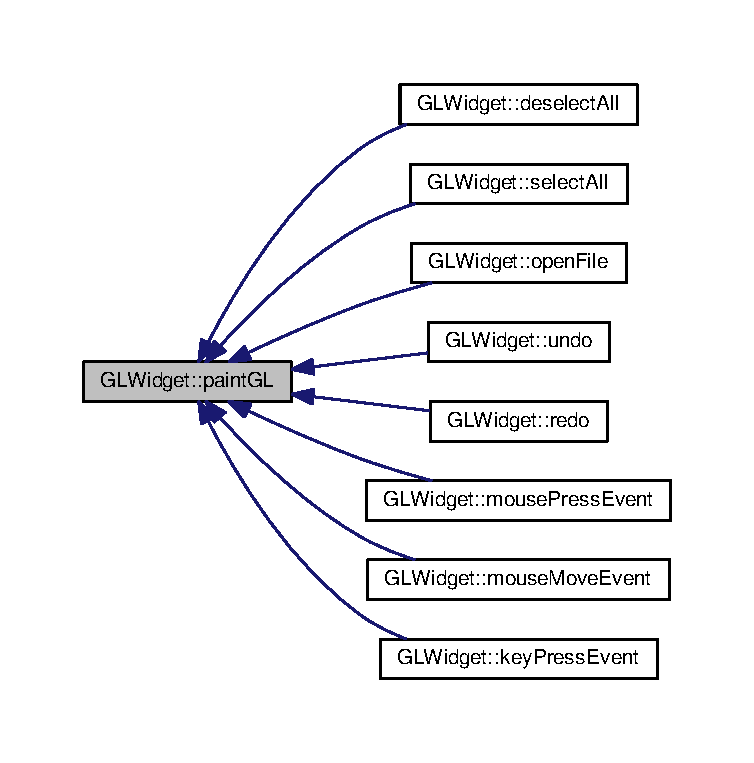
\includegraphics[width=350pt]{classGLWidget_a640b5570cb2b37724fd5b58a77339c5e_icgraph}
\end{center}
\end{figure}


\hypertarget{classGLWidget_a5371a80ec723e710374f302611710e15}{\index{G\-L\-Widget@{G\-L\-Widget}!redo@{redo}}
\index{redo@{redo}!GLWidget@{G\-L\-Widget}}
\subsubsection[{redo}]{\setlength{\rightskip}{0pt plus 5cm}void G\-L\-Widget\-::redo (
\begin{DoxyParamCaption}
{}
\end{DoxyParamCaption}
)}}\label{classGLWidget_a5371a80ec723e710374f302611710e15}


An implementation of redo. 

Moves the \#current\-State counter forward if it is less than the number of states that have been saved. \hypertarget{classGLWidget_ac0d2a8ecf60907a81c0d73475d851025}{\index{G\-L\-Widget@{G\-L\-Widget}!resize\-G\-L@{resize\-G\-L}}
\index{resize\-G\-L@{resize\-G\-L}!GLWidget@{G\-L\-Widget}}
\subsubsection[{resize\-G\-L}]{\setlength{\rightskip}{0pt plus 5cm}void G\-L\-Widget\-::resize\-G\-L (
\begin{DoxyParamCaption}
\item[{int}]{width, }
\item[{int}]{height}
\end{DoxyParamCaption}
)\hspace{0.3cm}{\ttfamily [protected]}}}\label{classGLWidget_ac0d2a8ecf60907a81c0d73475d851025}
Called whenever the widget is resized. Overrides resize\-G\-L in Q\-G\-L\-Widget \hypertarget{classGLWidget_aebdd7462523ecff734ac224031ec9e0b}{\index{G\-L\-Widget@{G\-L\-Widget}!save\-File@{save\-File}}
\index{save\-File@{save\-File}!GLWidget@{G\-L\-Widget}}
\subsubsection[{save\-File}]{\setlength{\rightskip}{0pt plus 5cm}bool G\-L\-Widget\-::save\-File (
\begin{DoxyParamCaption}
\item[{const std\-::string \&}]{file\-Name}
\end{DoxyParamCaption}
)}}\label{classGLWidget_aebdd7462523ecff734ac224031ec9e0b}


This will save a file {\ttfamily file\-Name} using Q\-Data\-Stream version (Qt 4.\-9). 

The \hyperlink{classGLWidget_a0ecdf8ea93e62ab9d294714e59dafd64}{dimension}, \hyperlink{classGLWidget_a272046b9cb9f26f5b382f9a121672570}{grid\-Width}, and \hyperlink{classGLWidget_a419c32eef067d7157b00904dd52bdb8b}{grid\-Height} are written first as qint32 integers. Then each red, green, blue, and alpha component of every Q\-Color in \hyperlink{classGLWidget_aab1b8762be4b33d384e3689427c2addc}{color\-Matrix} are written as qint32 integers.

\begin{DoxyReturn}{Returns}

\begin{DoxyItemize}
\item true if saving succeeded
\item false otherwise 
\end{DoxyItemize}
\end{DoxyReturn}
\hypertarget{classGLWidget_a9c9e2bd40c564a1e6a4df98960355b6e}{\index{G\-L\-Widget@{G\-L\-Widget}!save\-History\-State@{save\-History\-State}}
\index{save\-History\-State@{save\-History\-State}!GLWidget@{G\-L\-Widget}}
\subsubsection[{save\-History\-State}]{\setlength{\rightskip}{0pt plus 5cm}void G\-L\-Widget\-::save\-History\-State (
\begin{DoxyParamCaption}
{}
\end{DoxyParamCaption}
)\hspace{0.3cm}{\ttfamily [protected]}}}\label{classGLWidget_a9c9e2bd40c564a1e6a4df98960355b6e}


Saves the current state of the \hyperlink{classGLWidget}{G\-L\-Widget}. 

Will save the \hyperlink{classGLWidget_a272046b9cb9f26f5b382f9a121672570}{grid\-Width}, \hyperlink{classGLWidget_a419c32eef067d7157b00904dd52bdb8b}{grid\-Height}, \hyperlink{classGLWidget_a0ecdf8ea93e62ab9d294714e59dafd64}{dimension}, \hyperlink{classGLWidget_aab1b8762be4b33d384e3689427c2addc}{color\-Matrix}, and \hyperlink{classGLWidget_ab07a9ee710f42da54d0158cbdedf3674}{selected\-Bixels} into a \hyperlink{structGLWidget_1_1HistoryState}{History\-State} and push it into the history. This is called on every \hyperlink{classGLWidget_a3fff7f887bf2ab1df58c870fb6146f31}{key\-Release\-Event} as well as every \hyperlink{classGLWidget_ab992c4c25439a5ef23031991015451c1}{mouse\-Release\-Event}.

Currently the max number of states that can be saved is 99.

\begin{DoxySeeAlso}{See Also}
\hyperlink{structGLWidget_1_1HistoryState}{History\-State} 
\end{DoxySeeAlso}
\hypertarget{classGLWidget_abe918fd89a3f4c4f3d8864efee282610}{\index{G\-L\-Widget@{G\-L\-Widget}!select\-All@{select\-All}}
\index{select\-All@{select\-All}!GLWidget@{G\-L\-Widget}}
\subsubsection[{select\-All}]{\setlength{\rightskip}{0pt plus 5cm}void G\-L\-Widget\-::select\-All (
\begin{DoxyParamCaption}
{}
\end{DoxyParamCaption}
)}}\label{classGLWidget_abe918fd89a3f4c4f3d8864efee282610}
This will add every Bixel index to \hyperlink{classGLWidget_ab07a9ee710f42da54d0158cbdedf3674}{selected\-Bixels}. Calls \hyperlink{classGLWidget_a640b5570cb2b37724fd5b58a77339c5e}{paint\-G\-L}. \hypertarget{classGLWidget_ac41fdd4181036c79f4bdf688045155b3}{\index{G\-L\-Widget@{G\-L\-Widget}!select\-Bixel\-At@{select\-Bixel\-At}}
\index{select\-Bixel\-At@{select\-Bixel\-At}!GLWidget@{G\-L\-Widget}}
\subsubsection[{select\-Bixel\-At}]{\setlength{\rightskip}{0pt plus 5cm}void G\-L\-Widget\-::select\-Bixel\-At (
\begin{DoxyParamCaption}
\item[{int}]{i, }
\item[{int}]{j}
\end{DoxyParamCaption}
)}}\label{classGLWidget_ac41fdd4181036c79f4bdf688045155b3}
This will add a Bixel index ({\ttfamily i}, {\ttfamily j}) to \hyperlink{classGLWidget_ab07a9ee710f42da54d0158cbdedf3674}{selected\-Bixels} if it is not already selected. \hypertarget{classGLWidget_ab07a9ee710f42da54d0158cbdedf3674}{\index{G\-L\-Widget@{G\-L\-Widget}!selected\-Bixels@{selected\-Bixels}}
\index{selected\-Bixels@{selected\-Bixels}!GLWidget@{G\-L\-Widget}}
\subsubsection[{selected\-Bixels}]{\setlength{\rightskip}{0pt plus 5cm}std\-::set$<$ G\-L\-Widget\-::\-Color\-Matrix\-Index $>$ G\-L\-Widget\-::selected\-Bixels (
\begin{DoxyParamCaption}
{}
\end{DoxyParamCaption}
)}}\label{classGLWidget_ab07a9ee710f42da54d0158cbdedf3674}
Returns a set of all of the Bixels currently selected. This needs to be its own set because we want to quickly
\begin{DoxyItemize}
\item fill a selection with \hyperlink{classGLWidget_a1acd74645ffbe6bc071365c2bbd176ba}{fill\-Selected} without redrawing everything.
\item insert new selections without redrawing everything
\item remove selections without redrawing everything
\end{DoxyItemize}

Having each member of color\-Matrix have its own selection attribute would mean that we would have to redraw the entire screen everytime we selected or deselected. \begin{DoxySeeAlso}{See Also}
\hyperlink{classGLWidget_a9fba3eba78950865febd4547be0641d0a53197083abb268d80465c7af0071bfe7}{M\-O\-U\-S\-E} 
\end{DoxySeeAlso}
\hypertarget{classGLWidget_a0f0089107cb0fbe89b337dfc01384e28}{\index{G\-L\-Widget@{G\-L\-Widget}!select\-Rectangle@{select\-Rectangle}}
\index{select\-Rectangle@{select\-Rectangle}!GLWidget@{G\-L\-Widget}}
\subsubsection[{select\-Rectangle}]{\setlength{\rightskip}{0pt plus 5cm}void G\-L\-Widget\-::select\-Rectangle (
\begin{DoxyParamCaption}
\item[{const std\-::vector$<$ int $>$ \&}]{p1, }
\item[{const std\-::vector$<$ int $>$ \&}]{p2}
\end{DoxyParamCaption}
)}}\label{classGLWidget_a0f0089107cb0fbe89b337dfc01384e28}
Adds all Bixels within a rectangle between the {\ttfamily point1} and {\ttfamily point2} to the \hyperlink{classGLWidget_ab07a9ee710f42da54d0158cbdedf3674}{selected\-Bixels}. If either point is out of bounds, it will be set to the closest bixel that is in bounds.


\begin{DoxyParams}{Parameters}
{\em p1} & The top left corner of the rectangle to be selected. \\
\hline
{\em p2} & The bottom right corner of the rectangle to be selected. \\
\hline
\end{DoxyParams}
\hypertarget{classGLWidget_a5abf53a0389c884788c3c106a7a1263d}{\index{G\-L\-Widget@{G\-L\-Widget}!set\-Color\-At@{set\-Color\-At}}
\index{set\-Color\-At@{set\-Color\-At}!GLWidget@{G\-L\-Widget}}
\subsubsection[{set\-Color\-At}]{\setlength{\rightskip}{0pt plus 5cm}void G\-L\-Widget\-::set\-Color\-At (
\begin{DoxyParamCaption}
\item[{int}]{i, }
\item[{int}]{j, }
\item[{Q\-Color}]{color}
\end{DoxyParamCaption}
)}}\label{classGLWidget_a5abf53a0389c884788c3c106a7a1263d}
Sets a color at ({\ttfamily i}, {\ttfamily j}) in \hyperlink{classGLWidget_aab1b8762be4b33d384e3689427c2addc}{color\-Matrix} to {\ttfamily color}. \hypertarget{classGLWidget_a087325630069166821ada20445fc89a6}{\index{G\-L\-Widget@{G\-L\-Widget}!set\-Drawing\-Color@{set\-Drawing\-Color}}
\index{set\-Drawing\-Color@{set\-Drawing\-Color}!GLWidget@{G\-L\-Widget}}
\subsubsection[{set\-Drawing\-Color}]{\setlength{\rightskip}{0pt plus 5cm}void G\-L\-Widget\-::set\-Drawing\-Color (
\begin{DoxyParamCaption}
\item[{const Q\-Color \&}]{color}
\end{DoxyParamCaption}
)}}\label{classGLWidget_a087325630069166821ada20445fc89a6}
Sets the current drawing color used by B\-R\-U\-S\-H, P\-A\-I\-N\-T\-B\-U\-C\-K\-E\-T, and \hyperlink{classGLWidget_a1acd74645ffbe6bc071365c2bbd176ba}{fill\-Selected}. \begin{DoxySeeAlso}{See Also}
\hyperlink{classGLWidget_a8ea9c1e6b1013897e22dc7121f377113}{drawing\-Color()} 
\end{DoxySeeAlso}
\hypertarget{classGLWidget_ad7b5ee8248e47c8c1c9c1525c9e5acce}{\index{G\-L\-Widget@{G\-L\-Widget}!tool@{tool}}
\index{tool@{tool}!GLWidget@{G\-L\-Widget}}
\subsubsection[{tool}]{\setlength{\rightskip}{0pt plus 5cm}{\bf G\-L\-Widget\-::\-Draw\-Tool} G\-L\-Widget\-::tool (
\begin{DoxyParamCaption}
{}
\end{DoxyParamCaption}
)}}\label{classGLWidget_ad7b5ee8248e47c8c1c9c1525c9e5acce}
Returns the tool the user is currently using. \hypertarget{classGLWidget_aed44b9ce42449cf8f086a743bbbac7cd}{\index{G\-L\-Widget@{G\-L\-Widget}!undo@{undo}}
\index{undo@{undo}!GLWidget@{G\-L\-Widget}}
\subsubsection[{undo}]{\setlength{\rightskip}{0pt plus 5cm}void G\-L\-Widget\-::undo (
\begin{DoxyParamCaption}
{}
\end{DoxyParamCaption}
)}}\label{classGLWidget_aed44b9ce42449cf8f086a743bbbac7cd}


An implementation of the undo function. 

Moves the \#current\-State counter back one if the counter is greater than 0. This method calls \hyperlink{classGLWidget_a640b5570cb2b37724fd5b58a77339c5e}{paint\-G\-L}.

\begin{DoxyRefDesc}{Todo}
\item[\hyperlink{todo__todo000005}{Todo}]add Current\-State access method \end{DoxyRefDesc}


The documentation for this class was generated from the following files\-:\begin{DoxyCompactItemize}
\item 
src/glwidget.\-hpp\item 
src/glwidget.\-cpp\end{DoxyCompactItemize}

\hypertarget{structGLWidget_1_1HistoryState}{\section{G\-L\-Widget\-:\-:History\-State Struct Reference}
\label{structGLWidget_1_1HistoryState}\index{G\-L\-Widget\-::\-History\-State@{G\-L\-Widget\-::\-History\-State}}
}


This struct stores the current state of a \hyperlink{classGLWidget}{G\-L\-Widget}.  




{\ttfamily \#include $<$glwidget.\-hpp$>$}

\subsection*{Public Member Functions}
\begin{DoxyCompactItemize}
\item 
\hyperlink{structGLWidget_1_1HistoryState_ae299cd96c1489e61d82519333fc19294}{History\-State} (\hyperlink{classGLWidget}{G\-L\-Widget} $\ast$widget\-To\-Save)
\item 
\hypertarget{structGLWidget_1_1HistoryState_aa7b14b8891f4560d7ab1b6e9cc528777}{bool {\bfseries operator==} (\hyperlink{structGLWidget_1_1HistoryState}{History\-State} b)}\label{structGLWidget_1_1HistoryState_aa7b14b8891f4560d7ab1b6e9cc528777}

\end{DoxyCompactItemize}
\subsection*{Public Attributes}
\begin{DoxyCompactItemize}
\item 
\hypertarget{structGLWidget_1_1HistoryState_ae99febc3bc2759952e1870cd3413528d}{int {\bfseries dimension\-\_\-state}}\label{structGLWidget_1_1HistoryState_ae99febc3bc2759952e1870cd3413528d}

\item 
\hypertarget{structGLWidget_1_1HistoryState_a06668527759df59da44a53164526d581}{int {\bfseries grid\-Width\-\_\-state}}\label{structGLWidget_1_1HistoryState_a06668527759df59da44a53164526d581}

\item 
\hypertarget{structGLWidget_1_1HistoryState_a858a0163cdc7072a92b0bb1476d2ea00}{int {\bfseries grid\-Height\-\_\-state}}\label{structGLWidget_1_1HistoryState_a858a0163cdc7072a92b0bb1476d2ea00}

\item 
\hypertarget{structGLWidget_1_1HistoryState_abd095bfba5c17c91295db78686078096}{std\-::vector$<$ Q\-Color $>$ {\bfseries color\-Matrix\-\_\-state}}\label{structGLWidget_1_1HistoryState_abd095bfba5c17c91295db78686078096}

\item 
\hypertarget{structGLWidget_1_1HistoryState_a080e8b35ba02f2218038218f021a3cb2}{std\-::set$<$ int $>$ {\bfseries selected\-Bixels\-\_\-state}}\label{structGLWidget_1_1HistoryState_a080e8b35ba02f2218038218f021a3cb2}

\end{DoxyCompactItemize}


\subsection{Detailed Description}
This struct stores the current state of a \hyperlink{classGLWidget}{G\-L\-Widget}. 

The struct stores the width and height of the Bixel Grid, the dimension of the Bixel grid, the color of every Bixel, and all of the selected Bixels.

\begin{DoxySeeAlso}{See Also}
\hyperlink{classGLWidget}{G\-L\-Widget} 

\hyperlink{classGLWidget_a9c9e2bd40c564a1e6a4df98960355b6e}{G\-L\-Widget\-::save\-History\-State()} 

\hyperlink{classGLWidget_acb2ac0440f3e004a77c31f8b035fb8a4}{G\-L\-Widget\-::load\-History\-State(int)} 

\hyperlink{classGLWidget_aed44b9ce42449cf8f086a743bbbac7cd}{G\-L\-Widget\-::undo()} 

\hyperlink{classGLWidget_a5371a80ec723e710374f302611710e15}{G\-L\-Widget\-::redo()} 
\end{DoxySeeAlso}


\subsection{Constructor \& Destructor Documentation}
\hypertarget{structGLWidget_1_1HistoryState_ae299cd96c1489e61d82519333fc19294}{\index{G\-L\-Widget\-::\-History\-State@{G\-L\-Widget\-::\-History\-State}!History\-State@{History\-State}}
\index{History\-State@{History\-State}!GLWidget::HistoryState@{G\-L\-Widget\-::\-History\-State}}
\subsubsection[{History\-State}]{\setlength{\rightskip}{0pt plus 5cm}G\-L\-Widget\-::\-History\-State\-::\-History\-State (
\begin{DoxyParamCaption}
\item[{{\bf G\-L\-Widget} $\ast$}]{widget\-To\-Save}
\end{DoxyParamCaption}
)\hspace{0.3cm}{\ttfamily [inline]}}}\label{structGLWidget_1_1HistoryState_ae299cd96c1489e61d82519333fc19294}
The History state constructor takes a snapshot of the current Widget, saving all of the important attributes. 
\begin{DoxyParams}{Parameters}
{\em widget\-To\-Save} & A pointer to the widget to be saved. \\
\hline
\end{DoxyParams}


The documentation for this struct was generated from the following file\-:\begin{DoxyCompactItemize}
\item 
src/glwidget.\-hpp\end{DoxyCompactItemize}

\hypertarget{classSwatch}{\section{Swatch Class Reference}
\label{classSwatch}\index{Swatch@{Swatch}}
}


Inheritance diagram for Swatch\-:\nopagebreak
\begin{figure}[H]
\begin{center}
\leavevmode
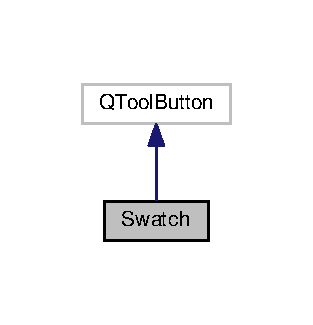
\includegraphics[width=150pt]{classSwatch__inherit__graph}
\end{center}
\end{figure}


Collaboration diagram for Swatch\-:\nopagebreak
\begin{figure}[H]
\begin{center}
\leavevmode
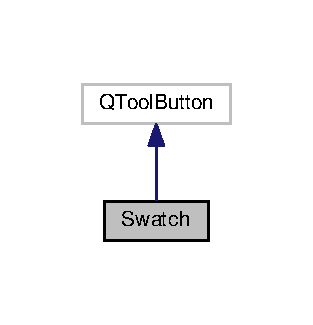
\includegraphics[width=150pt]{classSwatch__coll__graph}
\end{center}
\end{figure}
\subsection*{Signals}
\begin{DoxyCompactItemize}
\item 
\hypertarget{classSwatch_a4cc4620ddd05270f7c9a11addefcad57}{void {\bfseries swatch\-Picked} (const Q\-Color \&color)}\label{classSwatch_a4cc4620ddd05270f7c9a11addefcad57}

\end{DoxyCompactItemize}
\subsection*{Public Member Functions}
\begin{DoxyCompactItemize}
\item 
\hypertarget{classSwatch_ad411aab2ef21c65041939bfe3fe77b0e}{{\bfseries Swatch} (Q\-Widget $\ast$parent=0)}\label{classSwatch_ad411aab2ef21c65041939bfe3fe77b0e}

\item 
\hypertarget{classSwatch_a306fa88806e4b2d1fbf4e70f5878ae52}{void {\bfseries set\-Color} (Q\-Rgb color)}\label{classSwatch_a306fa88806e4b2d1fbf4e70f5878ae52}

\item 
\hypertarget{classSwatch_a53bfaa32646c4ee3555419f1edb5820d}{void {\bfseries set\-Color} (Q\-Color color)}\label{classSwatch_a53bfaa32646c4ee3555419f1edb5820d}

\item 
\hypertarget{classSwatch_aea70e9f1fd2b26b3e686b615b734d27a}{void {\bfseries set\-Color} (int r, int g, int b, int a=255)}\label{classSwatch_aea70e9f1fd2b26b3e686b615b734d27a}

\item 
\hypertarget{classSwatch_a6104b4c53efb97a496dd3554bf542ebb}{Q\-Color {\bfseries color} ()}\label{classSwatch_a6104b4c53efb97a496dd3554bf542ebb}

\end{DoxyCompactItemize}
\subsection*{Protected Member Functions}
\begin{DoxyCompactItemize}
\item 
\hypertarget{classSwatch_ab9aacb2c821dce15d22f54d34b68d023}{void {\bfseries mouse\-Release\-Event} (Q\-Mouse\-Event $\ast$)}\label{classSwatch_ab9aacb2c821dce15d22f54d34b68d023}

\end{DoxyCompactItemize}
\subsection*{Private Attributes}
\begin{DoxyCompactItemize}
\item 
\hypertarget{classSwatch_ac7c3eb52b20545b969f7aea97c985d5d}{Q\-Color {\bfseries m\-\_\-color}}\label{classSwatch_ac7c3eb52b20545b969f7aea97c985d5d}

\end{DoxyCompactItemize}


The documentation for this class was generated from the following files\-:\begin{DoxyCompactItemize}
\item 
src/swatch.\-hpp\item 
src/swatch.\-cpp\end{DoxyCompactItemize}

\hypertarget{classvec2}{\section{vec2 Class Reference}
\label{classvec2}\index{vec2@{vec2}}
}
\subsection*{Public Member Functions}
\begin{DoxyCompactItemize}
\item 
\hypertarget{classvec2_add5c0b4c7cf081d3292788a452cb489a}{{\bfseries vec2} (double x=0, double y=0)}\label{classvec2_add5c0b4c7cf081d3292788a452cb489a}

\item 
\hypertarget{classvec2_aedc685aecce22ebb9832a0dfa9ba4e76}{void {\bfseries set} (double x, double y)}\label{classvec2_aedc685aecce22ebb9832a0dfa9ba4e76}

\item 
\hypertarget{classvec2_a6e4d7583e07fd84b3314896e2f49f9c0}{\hyperlink{classvec2}{vec2} {\bfseries operator+} (const \hyperlink{classvec2}{vec2} \&b) const }\label{classvec2_a6e4d7583e07fd84b3314896e2f49f9c0}

\item 
\hypertarget{classvec2_afb69e05f24446157113eebf78b8fa64b}{\hyperlink{classvec2}{vec2} {\bfseries operator-\/} (const \hyperlink{classvec2}{vec2} \&b) const }\label{classvec2_afb69e05f24446157113eebf78b8fa64b}

\item 
\hypertarget{classvec2_aa9aacd2fc0ad8e81efe83e9f02b21749}{bool {\bfseries operator==} (const \hyperlink{classvec2}{vec2} \&b) const }\label{classvec2_aa9aacd2fc0ad8e81efe83e9f02b21749}

\end{DoxyCompactItemize}
\subsection*{Public Attributes}
\begin{DoxyCompactItemize}
\item 
\hypertarget{classvec2_ac38b8dcc3bc5eb2b4fb6971638af64d1}{double {\bfseries x}}\label{classvec2_ac38b8dcc3bc5eb2b4fb6971638af64d1}

\item 
\hypertarget{classvec2_a77fcc56ac7af5cee53b8ca789dacac1f}{double {\bfseries y}}\label{classvec2_a77fcc56ac7af5cee53b8ca789dacac1f}

\end{DoxyCompactItemize}


The documentation for this class was generated from the following files\-:\begin{DoxyCompactItemize}
\item 
src/vec2.\-hpp\item 
src/vec2.\-cpp\end{DoxyCompactItemize}

%--- End generated contents ---

% Index
\newpage
\phantomsection
\addcontentsline{toc}{chapter}{Index}
\printindex

\end{document}
